\documentclass[12pt,a4paper,oneside,openany]{book}

% --- Basic Setup & Spacing ---
\newcommand\tab[1][1cm]{\hspace*{#1}} % Custom tab command
\sloppy % Adjusts word spacing to avoid overfull hboxes, can lead to more varied spacing
\usepackage{xurl}
% --- Core Packages ---
\usepackage[english]{babel} % Language support
\usepackage[utf8]{inputenc} % Input encoding (often default in modern LaTeX)
\usepackage[T1]{fontenc}    % Output font encoding (for better hyphenation and special chars)
\usepackage[frozencache=false]{minted}

\usepackage{inconsolata} % A clean, modern monospaced font
\newcommand{\cframe}[1]{\colorbox{black!10}{\texttt{#1}}}

\usepackage{booktabs} 

% --- Page Layout & Geometry ---
\usepackage[left=1.2in,right=1.2in,top=1in,bottom=1in]{geometry}
\usepackage{setspace}


% --- Mathematics & Symbols ---
\usepackage{amsmath,amsthm,amssymb}

% --- Graphics & Colors ---
\usepackage{graphicx}
\usepackage{xcolor}

% --- Lists & Paragraphs ---
\usepackage{paralist} % For compact lists (consider replacing with enumitem's full power if needed)
\usepackage[inline]{enumitem} % For flexible inline and standard lists
\usepackage{tabularx}

% --- Code Listings ---
% For 'listings' package (if you use it as an alternative or for simple inline)
\usepackage{listings}

% --- Hyperlinks, URLs, Citations ---
\usepackage{url}      % For typesetting URLs
\usepackage{hyperref} % For clickable links and PDF metadata (load late)
\hypersetup{
    colorlinks=true,
    linkcolor=blue,
    filecolor=magenta,
    urlcolor=cyan,
    pdftitle={Your Thesis Title}, % Add your actual title
    pdfauthor={Valase Paul Mihai}, % Your name
    pdfsubject={Bachelor Thesis},
    pdfkeywords={C2, Go, React, Cybersecurity, Threat Emulation}, % Add keywords
    bookmarks=true,
    bookmarksopen=true
}
\usepackage{cite}     % For citation management (e.g., [1,2,3] or [SMW12])

% --- Fonts (Optional) ---
% \usepackage{sourcecodepro} % Example: Monospaced font for code if desired
% \usepackage{lmodern} % A common modern alternative to Computer Modern

% --- Other Utilities ---
\usepackage{hyphenat} % For better hyphenation control
\usepackage{algorithm, algpseudocode} % For writing algorithms
\usepackage{float} % For more control over float placement, e.g., [H] for figures

% --- Theorem-like Environments ---
\newtheorem{thm}{Theorem}[section]
\newtheorem{lem}[thm]{Lemma}
\theoremstyle{definition}
\newtheorem{defn}{Definition}[section]
\theoremstyle{remark}
\newtheorem{rem}{Remark}[section]
\newtheorem{exmp}{Example}[section]

% --- Minted Configuration ---
\setminted{
    frame=lines,        % Add a frame around code blocks
    framesep=2mm,       % Space between frame and code
    baselinestretch=1.0,% Line spacing within code
    fontsize=\footnotesize, % Font size for code
    linenos,            % Display line numbers
    breaklines,         % Allow automatic line breaks in long lines
    breakautoindent=true,% Indent continued lines
    tabsize=4,          % Tabulator size
    bgcolor=backcolour  % Background color for minted blocks
}
% Define background color for minted if not already defined by lstdefinestyle
\definecolor{backcolour}{rgb}{0.95,0.95,0.92}

% --- Listings Package Configuration (if used) ---
\definecolor{codegreen}{rgb}{0,0.6,0}
\definecolor{codegray}{rgb}{0.5,0.5,0.5}
\definecolor{codepurple}{rgb}{0.58,0,0.82}
% backcolour is already defined above

\lstdefinestyle{mystyle}{
    backgroundcolor=\color{backcolour},
    commentstyle=\color{codegreen},
    keywordstyle=\color{magenta},
    numberstyle=\tiny\color{codegray},
    stringstyle=\color{codepurple},
    basicstyle=\ttfamily\footnotesize,
    breakatwhitespace=false, % If true, breaks only at whitespace
    breaklines=true,         % Allow lines to break
    captionpos=b,            % Position of the caption (bottom)
    keepspaces=true,         % Keep spaces in the code
    numbers=left,            % Line numbers on the left
    numbersep=5pt,           % Space between line numbers and code
    showspaces=false,        % Don't show spaces as special characters
    showstringspaces=false,  % Don't show spaces in strings differently
    showtabs=false,          % Don't show tabs as special characters
    tabsize=2                % Tab size
}
\lstset{style=mystyle} % Set this as the default style for listings

% ==============================================================================
\begin{document}
% ==============================================================================

% --- FRONT MATTER ---
% Title Page 1 (University Standard)
\thispagestyle{empty}
\begin{center}

\includegraphics[width=100pt]{includegraphics/uvt_logo.png} \\[2cm] % Ensure this path is correct
{\large {\bf WEST UNIVERSITY OF TIMI\c SOARA \\
FACULTY OF MATHEMATICS AND COMPUTER SCIENCE \\
BACHELOR STUDY PROGRAM: COMPUTER SCIENCE IN ENGLISH}} \\[4cm]
{\huge {\bf BACHELOR THESIS}} \\[5cm]
{\large \bf SUPERVISOR: \hfill GRADUATE:} \\[0.5cm]
{\large lect. dr. Cristian Cira \hfill Valase Paul Mihai}
\end{center}
\vfill
\begin{center}
{\bf TIMI\c SOARA \\ 2025} % Update year if needed
\end{center}
\clearpage

% Title Page 2 (Thesis Specific)
\begin{titlepage}
\centering

\includegraphics[width=100pt]{includegraphics/uvt_logo.png} \\[2cm] % Ensure this path is correct
{\large \textbf{WEST UNIVERSITY OF TIMIŞOARA}} \\
\large \textbf{FACULTY OF MATHEMATICS AND COMPUTER SCIENCE} \\
\large \textbf{BACHELOR STUDY PROGRAM: COMPUTER SCIENCE IN ENGLISH} \\[2cm]
{\Huge \textbf{Development of a Command-and-Control (C2) Framework with Go-Based Implants and React Web Interface for Threat Emulation}} \\[1cm] % Updated Title
{\large \textbf{SUPERVISOR:} lect. dr. Cristian Cira} \\[0.5cm]
{\large \textbf{GRADUATE:} Valase Paul Mihai} \\[5cm]
{\large TIMIŞOARA \\ 2025} % Update year if needed
\end{titlepage}
\clearpage

% Optional: Declaration of Authenticity / Honesty
% \input{chapters/declaration}
% \clearpage

\pagenumbering{roman} % Roman numerals for front matter (ToC, Abstract, etc.)

% Abstract
\chapter*{Abstract}
\onehalfspacing
\addcontentsline{toc}{chapter}{Abstract} 

This bachelor thesis details the design, implementation, and evaluation of a Command-and-Control (C2) framework intended for cybersecurity research and threat emulation. The system comprises a C2 server developed in Go, leveraging the \verb|Gin Gonic framework| for robust API handling, and Go-based implants designed for stealth and multi-platform compatibility (Windows and Linux). A modern web-based client, built with React, provides operators with an intuitive interface for real-time implant (an implant is a malicious  management, command execution, filesystem interaction, and live desktop streaming.

The core objective is to provide a modular and extensible platform for simulating advanced attacker TTPs (Tactics, Techniques, and Procedures) in controlled environments. Implants incorporate features such as daemonization, self-deletion, process name manipulation, and secure communication with the C2 server. The thesis explores various evasion techniques employed by the implants to bypass common detection mechanisms.

The experimental validation demonstrates the framework's capabilities, including remote command execution, file system enumeration, screenshot capture, and basic evasion characteristics. This project contributes a functional C2 system that can aid security professionals in understanding adversarial methodologies, testing defensive postures, and improving overall cybersecurity resilience. Ethical considerations and responsible use for defensive purposes are emphasized throughout the research.
\clearpage

% Acknowledgements (Optional but good practice)
% \chapter*{Acknowledgements}
% \addcontentsline{toc}{chapter}{Acknowledgements}
% Your acknowledgements text here...
% \clearpage

\tableofcontents
\clearpage

% Optional: List of Figures, Tables, Listings
% \listoffigures
% \addcontentsline{toc}{chapter}{List of Figures}
% \clearpage

% \listoftables
% \addcontentsline{toc}{chapter}{List of Tables}
% \clearpage

% If using minted and want a list of listings
% \renewcommand{\listoflistingscaption}{List of Code Listings} % Custom title
% \listoflistings
% \addcontentsline{toc}{chapter}{List of Code Listings}
% \clearpage

\pagenumbering{arabic} % Arabic numerals for main content

% --- MAIN CONTENT ---
% ============================================================================
% CHAPTER 1: INTRODUCTION
% ============================================================================
\chapter{Introduction}
\label{chapter:introduction}

\section{ Motivation}
\label{sec:motivation}

The contemporary cybersecurity landscape is characterized by an escalating sophistication of threat actors who employ advanced persistent threats (APTs\footnote{ATP- Advanced Persistent Threats \textcolor{red}{se gfolofse la actori statali etc. pui un mic wiki}}) and complex attack methodologies to compromise organizational infrastructure \cite{hutchins2011intelligence}. Traditional security measures, while foundational, prove insufficient against adversaries who leverage Command and Control (C2) frameworks to maintain persistent access, exfiltrate sensitive data, and conduct reconnaissance activities within target networks \cite{caltagirone2013diamond}.

Educational institutions and cybersecurity practitioners require sophisticated tools to understand, analyze, and defend against these threats through controlled simulation and research. However, the current landscape of C2 frameworks presents significant challenges for academic and research applications. Commercial solutions such as Cobalt Strike\footnote{ce e asta} and Metasploit\footnote{some}, while technically advanced, impose financial constraints that limit accessibility for educational institutions and independent researchers \cite{red2019adversary}. Furthermore, these proprietary systems often lack the transparency necessary for academic scrutiny and pedagogical application.

Existing open-source alternatives, while accessible, frequently suffer from architectural limitations, inadequate documentation, and security vulnerabilities that compromise their utility for serious research endeavors \cite{mitre2023attack}. The absence of a comprehensive, academically-oriented C2 framework represents a significant gap in cybersecurity education and research infrastructure.

This research addresses these limitations by developing an advanced C2 framework that combines the sophistication required for realistic threat emulation with the transparency and extensibility necessary for academic application. The framework employs modern software engineering practices, incorporating microservices architecture, containerization, and contemporary web technologies to ensure scalability, maintainability, and educational value.

\section{Main Objectives}
\label{sec:objectives}

The primary objective of this research is to design, implement, and evaluate a comprehensive Command and Control framework suitable for cybersecurity research and educational applications. This overarching goal encompasses several specific technical and academic objectives:

\subsection{Primary Technical Objectives}

\begin{description}
\item[Architecture Design and Implementation] Develop a robust, scalable backend architecture utilizing the Go programming language and Gin web framework to handle concurrent connections from multiple implants while maintaining system stability and performance.

\item[Cross-Platform Implant Development] Create platform-agnostic implants capable of operating across Windows, Linux, and macOS environments, implementing essential C2 functionality including command execution, file system operations, and real-time communication.

\item[User Interface Development] Design and implement a responsive React-based web interface that provides intuitive access to C2 functionality while maintaining security through proper authentication and authorization mechanisms.

\item[Security Implementation] Integrate comprehensive security measures including encrypted communication channels, secure authentication protocols, and role-based access control to ensure operational security during research activities.

\item[Advanced Feature Integration]: Implement sophisticated capabilities such as real-time desktop streaming, comprehensive file system exploration, process management, and screenshot capture to enable realistic threat emulation scenarios.
\end{description}

\subsection{Academic and Research Objectives}

\begin{enumerate}
\item \textbf{Educational Framework Development}: Create comprehensive documentation, tutorials, and educational materials to facilitate the framework's adoption in academic curricula and cybersecurity training programs.

\item \textbf{Performance Evaluation}: Conduct systematic performance analysis to establish baseline metrics for latency, throughput, and scalability under various operational conditions.

\item \textbf{Security Analysis}: Perform comprehensive security assessment of the developed framework to identify potential vulnerabilities and establish best practices for secure deployment.

\item \textbf{Open Source Contribution}: Release the framework under an appropriate open-source license to encourage community collaboration and academic scrutiny.
\end{enumerate}

\section{Problem Statement}
\label{sec:problem_statement}

The current state of Command and Control frameworks presents several critical challenges that impede effective cybersecurity research and education: \textcolor{red}{foloseste description}

\begin{enumerate}

\item \textbf{Accessibility Constraints}: Commercial C2 frameworks impose significant financial barriers that limit access for educational institutions, independent researchers, and small security teams. This economic barrier creates an artificial scarcity of tools necessary for comprehensive cybersecurity education.

\item \textbf{Transparency Deficits}: Proprietary solutions lack the source code transparency required for academic analysis, peer review, and educational application. This opacity prevents students and researchers from understanding the underlying mechanisms that govern C2 operations.

\item \textbf{Technical Limitations}: Existing open-source alternatives often suffer from architectural deficiencies, including poor scalability, limited cross-platform support, and inadequate security implementations that compromise their utility for serious research applications.

\item \textbf{Documentation Inadequacy}: Available frameworks frequently lack comprehensive documentation, setup guides, and educational materials necessary for effective adoption in academic environments.

\item \textbf{Ethical Considerations}: Many existing tools are designed primarily for offensive operations without adequate consideration of ethical usage guidelines, responsible disclosure practices, or educational safeguards.
\end{enumerate}

\section{Contributions}
\label{sec:contributions}

This research makes several significant contributions to the cybersecurity community and academic domain:

\subsection{Technical Contributions}

\begin{enumerate}
\item \textbf{Modern Architecture Implementation}: Development of a microservices-based C2 architecture that separates concerns between command execution, data management, and user interface components, resulting in improved maintainability and scalability compared to monolithic alternatives.

\item \textbf{Cross-Platform Compatibility}: Creation of Go-based implants that leverage the language's cross-compilation capabilities to provide consistent functionality across diverse operating system environments without requiring platform-specific modifications.

\item \textbf{Real-Time Communication Protocols}: Implementation of efficient, low-latency communication mechanisms that enable real-time interaction between C2 infrastructure and deployed implants while maintaining security and reliability.

\item \textbf{Advanced Security Integration}: Development of comprehensive security mechanisms including JWT-based authentication, encrypted communication channels, and role-based authorization systems specifically tailored for C2 operations.
\end{enumerate}

\subsection{Academic Contributions}

\begin{enumerate}
\item \textbf{Educational Framework}: Creation of a comprehensive educational platform that includes detailed documentation, setup guides, and pedagogical materials suitable for cybersecurity curricula at undergraduate and graduate levels.

\item \textbf{Open Source Initiative}: Release of a fully functional, well-documented C2 framework under an open-source license, enabling community collaboration and academic scrutiny while maintaining ethical usage guidelines.

\item \textbf{Performance Benchmarking}: Establishment of performance baselines and scalability metrics that can serve as reference points for future C2 framework development and comparative analysis.

\item \textbf{Security Best Practices}: Documentation of security implementation patterns and best practices specifically applicable to C2 framework development and deployment in research environments.
\end{enumerate}

\section{Ethical Considerations}
\label{sec:ethics}

The development and dissemination of Command and Control frameworks raise significant ethical considerations that must be addressed throughout the research process. This project adheres to the principle of responsible disclosure and ethical cybersecurity research practices established by academic institutions and professional organizations.

\subsection{Responsible Development Principles}

\begin{enumerate}
\item \textbf{Educational Focus}: The framework is designed primarily for educational and research purposes, with built-in safeguards and documentation that emphasize legal and ethical usage scenarios.

\item \textbf{Controlled Testing Environment}: All development and testing activities are conducted within isolated laboratory environments, preventing potential impact on external systems or networks.

\item \textbf{Documentation of Limitations}: Clear documentation of framework limitations and security considerations to prevent misuse while enabling legitimate research activities.

\item \textbf{Community Oversight}: Open-source development model that enables community review and collaborative improvement of security features and ethical guidelines.
\end{enumerate}

\subsection{Legal and Regulatory Compliance}

This research complies with applicable laws and regulations governing cybersecurity research, including:

\begin{itemize}
\item Adherence to institutional review board (IRB) guidelines for research involving computer systems
\item Compliance with local and international laws regarding cybersecurity tool development and distribution
\item Implementation of appropriate use policies and access controls to prevent unauthorized usage
\item Establishment of clear guidelines for responsible disclosure of any vulnerabilities discovered during development
\end{itemize}

\section{Thesis Structure}
\label{sec:structure}

This thesis is organized into eight chapters that systematically present the research methodology, implementation details, and evaluation results:
\begin{description}

\item[Chapter 1 - Introduction] provides the research motivation, objectives, problem statement, and ethical considerations that guide this work.

\item[Chapter 2 - Background and Terminology] establishes the theoretical foundation by reviewing fundamental concepts in Command and Control frameworks, network security, and threat modeling methodologies.

\item[Chapter 3 - State of the Art] presents a comprehensive analysis of existing C2 frameworks, examining their architectural approaches, capabilities, limitations, and applicability to research environments.

\item[Chapter 4 - System Design and Architecture] details the architectural decisions, design patterns, and technological choices that inform the framework implementation.

\item[Chapter 5 - Implementation] provides detailed technical descriptions of the framework components, including backend services, implant development, and user interface implementation.

\item[Chapter 6 - Experimental Setup and Evaluation] describes the testing methodology, performance metrics, and evaluation criteria used to assess framework capabilities.

\item[Chapter 7 - Results and Analysis] presents the experimental results, performance analysis, and comparative evaluation against existing solutions.

\item[Chapter 8 - Discussion and Security Implications] analyzes the broader implications of the research, discusses security considerations, and addresses potential limitations and future improvements.

\item[Chapter 9 - Conclusion and Future Work] summarizes the research contributions, discusses limitations, and outlines directions for future development and research.
\end{description}


\chapter{Background and Terminology}
\label{chap:background}

This chapter introduces fundamental concepts and terminology essential for understanding the domain of Command-and-Control frameworks and threat emulation.

\section{Command-and-Control (C2/C\&C)}
\label{sec:c2_definition}
A Command-and-Control (C2 or C\&C) server is a centralized computer or system managed by an attacker (or, in ethical contexts, a security researcher/red teamer). Its primary purpose is to maintain communication with compromised systems, known as \textit{implants} or \textit{agents}, within a target network. Through the C2 channel, operators can send commands to implants, receive data, and orchestrate activities on the compromised hosts. The MITRE ATT\&CK framework lists Command and Control (TA0011) as a critical tactic used by adversaries \cite{mitreATTACK_C2}.

\section{Implant / Agent / Beacon}
\label{sec:implant_definition}
An \textit{implant} (also referred to as an agent, beacon, bot, or backdoor) is a malicious (or emulated malicious) program installed on a target system. Once active, the implant establishes a connection back to the C2 server, allowing the operator to remotely control the system. Key characteristics often include:
\begin{itemize}
    \item \textbf{Beaconing:} Periodically contacting the C2 server to check for new tasks or send status updates. The implant developed in this thesis performs check-ins every 5 seconds.
    \item \textbf{Task Execution:} Receiving and executing commands from the C2 server, such as running shell commands, manipulating files, or gathering system information.
    \item \textbf{Stealth:} Employing techniques to avoid detection by security software and analysts.
\end{itemize}
In this project, implants are developed in Go for cross-platform compatibility and performance.

\section{Payload}
\label{sec:payload_definition}
A \textit{payload} is the component of malware (or an emulation tool) that performs the intended malicious action. This can range from data exfiltration, encrypting files (ransomware), to establishing a persistent backdoor. In the context of C2 frameworks, the implant itself can be considered the primary payload delivered after initial access. The C2 server in this thesis facilitates the generation and configuration of these Go-based implant payloads.

\section{Threat Emulation vs. Penetration Testing}
\label{sec:emulation_vs_pentest}
While related, these terms have distinct meanings:
\textcolor{red}{descrioption}
\begin{itemize}
    \item \textbf{Penetration Testing:} Typically focuses on identifying and exploiting vulnerabilities to gain access, often with a broad scope and less emphasis on mimicking specific adversaries.
    \item \textbf{Threat Emulation (or Adversary Emulation):} A more targeted approach that seeks to replicate the specific Tactics, Techniques, and Procedures (TTPs) of known threat actors or attack scenarios. This project aims to provide a tool for threat emulation.
\end{itemize}

\section{Common C2 Communication Channels}
\label{sec:c2_channels}
Attackers use various protocols for C2 communication, often choosing common ones to blend in with legitimate traffic:
\begin{itemize}
    \item \textbf{HTTP/HTTPS:} Widely used due to its prevalence. The C2 framework in this thesis primarily uses HTTP for communication between implants and the server.
    \item \textbf{DNS:} Can be used for C2 by encoding data in DNS queries and responses.
    \item \textbf{ICMP:} Another common protocol that can be abused for covert channels.
    \item \textbf{Social Media/Cloud Services:} Abusing legitimate platforms like Twitter, Gmail, Dropbox, etc.
\end{itemize}

\section{Evasion Techniques}
\label{sec:evasion_techniques_intro}
These are methods used by malware and C2 implants to avoid detection by antivirus (AV) software, Endpoint Detection and Response (EDR) solutions, and security analysts. This thesis explores basic evasion techniques such as:
\begin{itemize}
    \item \textbf{Daemonization/Backgrounding:} Running the implant as a background process without a visible window or console. Your implant uses `relaunchAsDaemonInternal`.
    \item \textbf{Self-Deletion:} Removing the initial launcher or the implant binary from disk after execution to reduce forensic artifacts. Your implant implements `doSelfDelete`.
    \item \textbf{Process Name Spoofing/Masquerading:} Renaming the implant process to mimic a legitimate system process. Your Linux implant uses `prctl` and argv[0] manipulation.
    \item \textbf{In-Memory Execution:} Techniques to load and run code directly in memory without writing to disk (partially achieved by your Linux implant's copy-to-temp, exec, unlink).
    % \item \textbf{API Unhooking:} (Mentioned as future work) Restoring original API functions that EDRs might have hooked for monitoring.
    % \item \textbf{Process Injection:} (Mentioned as future work) Injecting malicious code into legitimate processes.
\end{itemize}
The MITRE ATT\&CK framework extensively documents Defense Evasion (TA0005) techniques \cite{mitreATTACK_DefenseEvasion}.

\section{MITRE ATT\&CK Framework}
\label{sec:mitre_attack}
The MITRE ATT\&CK\textsuperscript{\textregistered} framework is a globally accessible knowledge base of adversary tactics and techniques based on real-world observations. It is widely used by cybersecurity professionals for threat modeling, detection engineering, and improving security posture. This thesis aligns with several ATT\&CK tactics, primarily:
\begin{itemize}
    \item \textbf{Execution (TA0002):} e.g., Scheduled Task/Job (T1053), Command and Scripting Interpreter (T1059).
    \item \textbf{Persistence (TA0003):} e.g., Create or Modify System Process (T1543) through daemonization.
    \item \textbf{Defense Evasion (TA0005):} e.g., Masquerading (T1036), File Deletion (T1070.004).
    \item \textbf{Discovery (TA0007):} e.g., File and Directory Discovery (T1083), System Information Discovery (T1082).
    \item \textbf{Collection (TA0009):} e.g., Screen Capture (T1113).
    \item \textbf{Command and Control (TA0011):} e.g., Application Layer Protocol (T1071 - Web Protocols for your HTTP C2).
\end{itemize}
% ============================================================================
% CHAPTER 3: STATE OF THE ART
% ============================================================================
\chapter{State of the Art}
\label{chapter:state_of_art}

\section{Introduction}
\label{sec:sota_introduction}

The evolution of Command and Control (C2) frameworks represents a critical domain within cybersecurity research, encompassing both offensive security tools and defensive analysis capabilities. This chapter provides a comprehensive analysis of the current state of the art in C2 framework development, examining existing solutions, their architectural approaches, and their contributions to the cybersecurity research community.

The systematic review presented herein serves multiple purposes: first, to establish the theoretical and practical foundation upon which this research builds; second, to identify gaps and limitations in existing solutions that justify the development of a novel framework; and third, to position the contributions of this thesis within the broader context of cybersecurity research and tool development.

Contemporary C2 frameworks can be categorized into three primary classifications: commercial solutions designed for professional penetration testing and red team operations, open-source frameworks developed by the security research community, and academic prototypes created for educational and research purposes. Each category exhibits distinct characteristics in terms of functionality, accessibility, documentation quality, and intended use cases.

\section{Taxonomy of Command and Control Frameworks}
\label{sec:c2_taxonomy}

\subsection{Commercial C2 Solutions}
\label{subsec:commercial_solutions}

Commercial Command and Control frameworks represent the most mature and feature-complete solutions available in the cybersecurity market. These platforms typically offer comprehensive post-exploitation capabilities, sophisticated evasion techniques, and professional support structures.

\subsubsection{Cobalt Strike}

\textbf{Cobalt Strike}, developed by Strategic Cyber LLC, stands as the de facto standard for commercial C2 operations \cite{mudge2012cobalt}. The framework employs a client-server architecture where operators connect to a team server that manages implant communications. Key architectural features include:

\begin{itemize}
\item \textbf{Beacon Technology}: Utilizes HTTP/HTTPS beaconing with jitter and sleep intervals to evade network detection
\item \textbf{Malleable Profiles}: Customizable communication profiles that modify network traffic characteristics
\item \textbf{Lateral Movement}: Built-in capabilities for privilege escalation and network traversal
\item \textbf{Evasion Techniques}: Advanced anti-forensic and anti-analysis features
\end{itemize}

The framework's strength lies in its mature feature set and extensive documentation. However, its commercial licensing model (approximately \$3,500 per user annually) creates significant barriers for academic institutions and independent researchers \cite{rapid7_2023_cs}.

Metasploit Pro

The commercial variant of the Metasploit Framework extends the open-source foundation with enterprise-grade features including automated exploitation, advanced reporting, and team collaboration capabilities \cite{kennedy2011metasploit}. While primarily focused on vulnerability exploitation rather than C2 operations, its post-exploitation modules provide valuable insights into implant management architectures.

\subsection{Open-Source C2 Frameworks}
\label{subsec:opensource_solutions}

The open-source community has developed numerous C2 frameworks that address the accessibility limitations of commercial solutions while providing transparency for research applications.

\subsubsection{Sliver}

Sliver, developed by Bishop Fox, represents a modern approach to open-source C2 development \cite{bishopfox2022sliver}. Written in Go, the framework emphasizes cross-platform compatibility and operational security:

\begin{itemize}
\item \textbf{Multi-Platform Support}: Native implants for Windows, macOS, and Linux
\item \textbf{Multiple Protocols}: HTTP(S), DNS, and TCP communication channels
\item \textbf{Multiplayer Support}: Team server architecture supporting multiple operators
\item \textbf{Modern Architecture}: Utilizes gRPC for client-server communication
\end{itemize}

The framework's adoption of modern software engineering practices, including continuous integration and comprehensive testing, sets a high standard for open-source C2 development.

\subsubsection{Covenant}

Covenant, developed by Cobbr, implements a C2 framework using Microsoft's .NET ecosystem \cite{cobbr2019covenant}. The framework's architecture demonstrates several innovative approaches:

\begin{itemize}
\item \textbf{Web-Based Interface}: React.js frontend with ASP.NET Core backend
\item \textbf{Entity Framework Integration}: Database-first approach for data persistence
\item \textbf{Role-Based Access Control}: Multi-user support with granular permissions
\item \textbf{Docker Deployment}: Containerized deployment for simplified setup
\end{itemize}

Covenant's emphasis on user experience and deployment simplicity makes it particularly suitable for educational environments.

\subsubsection{Mythic}

Mythic framework, developed by its-a-feature, introduces a microservices architecture that separates C2 functionality into distinct components \cite{mythic2021framework}:

\begin{itemize}
\item \textbf{Agent-Agnostic Design}: Support for multiple implant types and languages
\item \textbf{Container-Based Architecture}: Each agent type runs in isolated containers
\item \textbf{Web Interface}: Modern React-based user interface
\item \textbf{Collaborative Features}: Multi-operator support with real-time collaboration
\end{itemize}

This architectural approach demonstrates the potential for modular C2 design, though the complexity of deployment and configuration may limit adoption in academic settings.

\subsubsection{Havoc}

\cframe{Havoc}, a recently developed open-source framework, focuses on providing enterprise-grade features while maintaining accessibility \cite{havoc2022framework}. Key characteristics include:

\begin{itemize}
\item \textbf{Modern UI/UX}: Qt-based client interface with professional aesthetics
\item \textbf{Lua Scripting}: Extensible functionality through scripting interfaces
\item \textbf{Advanced Evasion}: Built-in techniques for bypassing security controls
\item \textbf{Cross-Platform}: Support for multiple operating systems and architectures
\end{itemize}

\subsection{Academic and Research Prototypes}
\label{subsec:academic_solutions}

Academic contributions to C2 framework development often focus on specific research questions or novel architectural approaches rather than comprehensive operational capabilities.

\subsubsection{Research-Oriented Frameworks}

Several academic institutions have developed C2 frameworks for research purposes, though few have achieved widespread adoption due to limited documentation and support. Notable examples include university-based projects that explore specific aspects of C2 operations, such as communication protocols, evasion techniques, or detection methodologies.

\section{Architectural Analysis}
\label{sec:architectural_analysis}

\subsection{Communication Architectures}
\label{subsec:communication_architectures}

Contemporary C2 frameworks employ diverse communication architectures, each with distinct advantages and limitations:

\subsubsection{Client-Server Architecture}

The traditional client-server model, exemplified by \cframe{Cobalt Strike} and \cframe{Sliver}, centralizes command distribution and result collection through a dedicated server component. This approach offers several advantages:

\begin{itemize}
\item \textbf{Centralized Management}: Single point of control for multiple implants
\item \textbf{Scalability}: Efficient handling of large numbers of concurrent connections
\item \textbf{Logging and Auditing}: Comprehensive tracking of all C2 activities
\end{itemize}

However, the centralized architecture also presents potential vulnerabilities, as the discovery and disruption of the C2 server can compromise the entire operation.

\subsubsection{Peer-to-Peer Architecture}

Some advanced frameworks implement peer-to-peer communication models where implants can communicate directly with each other, creating redundant communication paths. This approach enhances resilience but increases complexity in implementation and management.

\subsubsection{Hybrid Architectures}

Modern frameworks increasingly adopt hybrid approaches that combine multiple communication methods, allowing operators to select the most appropriate protocol based on operational requirements and environmental constraints.

\subsection{User Interface Paradigms}
\label{subsec:ui_paradigms}

The evolution of C2 framework user interfaces reflects broader trends in software development and user experience design:

\subsubsection{Command-Line Interfaces}

Early C2 frameworks relied primarily on command-line interfaces, which while powerful, required significant technical expertise and limited collaborative capabilities.

\subsubsection{Desktop Applications}

Frameworks like \cframe{Cobalt Strike} and \cframe{Havoc} utilize desktop applications that provide rich functionality while maintaining responsive performance for real-time operations.

\subsubsection{Web-Based Interfaces}

The trend toward web-based interfaces, as demonstrated by \cframe{Covenant} and \cframe{Mythic}, offers several advantages:

\begin{itemize}
\item \textbf{Cross-Platform Compatibility}: Access from any system with a web browser
\item \textbf{Collaborative Features}: Multiple operators can work simultaneously
\item \textbf{Modern UI/UX}: Leveraging contemporary web development frameworks
\item \textbf{Deployment Simplicity}: Reduced client-side installation requirements
\end{itemize}

\section{Gap Analysis and Research Opportunities}
\label{sec:gap_analysis}

\subsection{Identified Limitations}
\label{subsec:identified_limitations}

The analysis of existing C2 frameworks reveals several significant limitations that present opportunities for research and development:

\subsubsection{Educational Accessibility}

Many existing frameworks lack comprehensive educational materials, making them difficult to adopt in academic settings. This limitation is particularly pronounced in:

\begin{itemize}
\item \textbf{Documentation Quality}: Insufficient technical documentation and setup guides
\item \textbf{Learning Resources}: Absence of tutorials and educational examples
\item \textbf{Code Clarity}: Complex codebases without adequate commenting or explanation
\end{itemize}

\subsubsection{Deployment Complexity}

Several open-source frameworks require extensive technical knowledge for proper deployment and configuration, creating barriers for users who wish to focus on research rather than system administration.

\subsubsection{Security Implementation}

Many frameworks lack comprehensive security implementations, particularly in areas such as:

\begin{itemize}
\item \textbf{Authentication and Authorization}: Basic or absent user management systems
\item \textbf{Communication Security}: Inadequate encryption or certificate management
\item \textbf{Audit Logging}: Limited tracking of user actions and system events
\end{itemize}

\subsubsection{Performance and Scalability}

Few frameworks provide detailed performance analysis or scalability testing, making it difficult to assess their suitability for large-scale research or educational deployments.

\subsection{Research Opportunities}
\label{subsec:research_opportunities}

The identified limitations suggest several areas where this research can make meaningful contributions:

\begin{enumerate}
\item \textbf{Educational Framework Development}: Creating a C2 framework specifically designed for academic use with comprehensive educational materials
\item \textbf{Modern Architecture Implementation}: Leveraging contemporary software engineering practices and technologies
\item \textbf{Security-First Design}: Implementing comprehensive security measures from the initial design phase
\item \textbf{Performance Optimization}: Conducting systematic performance analysis and optimization
\item \textbf{Deployment Simplification}: Utilizing containerization and automation for simplified setup
\end{enumerate}

\section{Methodological Influences}
\label{sec:methodological_influences}

\subsection{Software Engineering Practices}
\label{subsec:software_engineering}

Contemporary C2 framework development increasingly adopts modern software engineering practices:

\subsubsection{Containerization}

Frameworks like \cframe{Covenant} and \cframe{Mythic} utilize Docker containerization to simplify deployment and ensure consistent runtime environments. This approach offers several advantages for research and educational applications:

\begin{itemize}
\item \textbf{Reproducible Deployments}: Consistent behavior across different systems
\item \textbf{Isolation}: Separation of framework components from host systems
\item \textbf{Scalability}: Easy horizontal scaling of framework components
\end{itemize}

\subsubsection{Microservices Architecture}

The adoption of microservices patterns, particularly evident in \cframe{Mythic}, demonstrates the potential for modular C2 design that separates concerns and enables independent development of framework components.

\subsubsection{Continuous Integration and Testing}

Leading frameworks increasingly adopt CI/CD practices, automated testing, and code quality assurance measures that enhance reliability and maintainability.

\subsection{User Experience Design}
\label{subsec:ux_design}

The evolution toward modern user interfaces reflects the growing recognition that effective C2 operations require intuitive and efficient user experiences. Key trends include:

\begin{itemize}
\item \textbf{Responsive Design}: Interfaces that adapt to different screen sizes and devices
\item \textbf{Real-Time Updates}: Live updating of implant status and command results
\item \textbf{Collaborative Features}: Support for multiple simultaneous users
\item \textbf{Accessibility}: Design considerations for users with different abilities
\end{itemize}

\section{Technology Stack Analysis}
\label{sec:technology_analysis}

\subsection{Backend Technologies}
\label{subsec:backend_technologies}

Contemporary C2 frameworks employ diverse backend technologies, each with specific advantages:

\subsubsection{Go}

\cframe{Sliver} demonstrates the effectiveness of Go for C2 development, offering:
\begin{itemize}
\item \textbf{Cross-Platform Compilation}: Single codebase for multiple architectures
\item \textbf{Concurrency}: Built-in goroutines for handling multiple connections
\item \textbf{Static Binaries}: Self-contained executables without external dependencies
\item \textbf{Performance}: Compiled language with efficient memory management
\end{itemize}

\subsubsection{.NET Core}

\cframe{Covenant}'s use of .NET Core illustrates the platform's suitability for enterprise-grade C2 development:
\begin{itemize}
\item \textbf{Cross-Platform}: Support for Windows, macOS, and Linux
\item \textbf{Rich Ecosystem}: Extensive library support and tooling
\item \textbf{Entity Framework}: Sophisticated ORM for database operations
\item \textbf{Security Features}: Built-in authentication and authorization frameworks
\end{itemize}

\subsubsection{Python}

\cframe{Mythic} and several research frameworks utilize Python for rapid prototyping and development:
\begin{itemize}
\item \textbf{Development Speed}: Rapid iteration and prototyping capabilities
\item \textbf{Library Ecosystem}: Extensive third-party libraries for specialized functionality
\item \textbf{Scripting Integration}: Easy integration with automation and analysis tools
\end{itemize}

\subsection{Frontend Technologies}
\label{subsec:frontend_technologies}

Modern C2 frameworks increasingly adopt contemporary web technologies for user interface development:

\subsubsection{React.js}

Frameworks like \cframe{Covenant} and \cframe{Mythic} leverage React.js for building responsive, interactive user interfaces that provide:
\begin{itemize}
\item \textbf{Component-Based Architecture}: Reusable UI components for consistent design
\item \textbf{State Management}: Efficient handling of application state and updates
\item \textbf{Ecosystem}: Rich ecosystem of libraries and development tools
\end{itemize}

\subsubsection{Desktop Frameworks}

Traditional desktop frameworks (Qt, Electron) continue to be relevant for applications requiring high performance or offline capabilities.

\section{Security Considerations in Existing Frameworks}
\label{sec:security_considerations}

\subsection{Communication Security}
\label{subsec:communication_security}

Analysis of existing frameworks reveals varying approaches to securing C2 communications:

\subsubsection{Encryption Implementation}

Most modern frameworks implement TLS encryption for HTTP-based communications, though the quality and configuration of these implementations vary significantly. Key considerations include:

\begin{itemize}
\item \textbf{Certificate Management}: Approaches to handling TLS certificates in operational environments
\item \textbf{Cipher Suite Selection}: Choice of cryptographic algorithms and their security implications
\item \textbf{Perfect Forward Secrecy}: Implementation of PFS to protect historical communications
\end{itemize}

\subsubsection{Traffic Obfuscation}

Advanced frameworks implement various techniques to disguise C2 traffic:

\begin{itemize}
\item \textbf{Domain Fronting}: Utilizing CDN services to hide actual C2 servers
\item \textbf{Protocol Mimicry}: Disguising C2 traffic as legitimate protocols
\item \textbf{Steganography}: Hiding commands and data within seemingly benign content
\end{itemize}

\subsection{Access Control and Authentication}
\label{subsec:access_control}

Contemporary frameworks demonstrate varying sophistication in user management:

\subsubsection{Authentication Mechanisms}

\begin{itemize}
\item \textbf{Token-Based Authentication}: JWT and similar approaches for stateless authentication
\item \textbf{Multi-Factor Authentication}: Integration with external authentication providers
\item \textbf{Certificate-Based Authentication}: Client certificates for enhanced security
\end{itemize}

\subsubsection{Authorization Models}

\begin{itemize}
\item \textbf{Role-Based Access Control}: Different permission levels for different user types
\item \textbf{Attribute-Based Access Control}: Fine-grained permissions based on user attributes
\item \textbf{Audit Logging}: Comprehensive tracking of user actions for accountability
\end{itemize}

\section{Performance and Scalability Analysis}
\label{sec:performance_analysis}

\subsection{Benchmarking Methodologies}
\label{subsec:benchmarking}

Limited public research exists on the systematic performance evaluation of C2 frameworks. Available studies typically focus on specific aspects such as:

\begin{itemize}
\item \textbf{Connection Handling}: Maximum number of concurrent implant connections
\item \textbf{Command Latency}: Time between command issuance and execution
\item \textbf{Data Throughput}: Efficiency of large file transfers and data exfiltration
\item \textbf{Resource Utilization}: CPU, memory, and network resource consumption
\end{itemize}

\subsection{Scalability Challenges}
\label{subsec:scalability_challenges}

Analysis of existing frameworks reveals common scalability limitations:

\begin{itemize}
\item \textbf{Database Performance}: Bottlenecks in data storage and retrieval operations
\item \textbf{Network Handling}: Limitations in concurrent connection management
\item \textbf{User Interface Responsiveness}: Performance degradation with large numbers of implants
\item \textbf{Resource Consumption}: Inefficient memory or CPU utilization patterns
\end{itemize}

\section{Synthesis and Research Positioning}
\label{sec:synthesis}

\subsection{Framework Comparison Matrix}
\label{subsec:comparison_matrix}

Table~\ref{tab:framework_comparison} presents a systematic comparison of major C2 frameworks across key dimensions relevant to this research.

\begin{table}[htbp]
\centering
\caption{Comparison of Major C2 Frameworks}
\label{tab:framework_comparison}
\begin{tabularx}{\textwidth}{l|X|X|X|X|X}
\toprule
\textbf{Framework} & \textbf{License} & \textbf{Architecture} & \textbf{UI Type} & \textbf{Documentation} & \textbf{Educational Use} \\
\midrule
Cobalt Strike & Commercial & Client-Server & Desktop & Excellent & Limited \\
Sliver & Open Source & Client-Server & CLI/Web & Good & Moderate \\
Covenant & Open Source & Web-Based & Web & Good & High \\
Mythic & Open Source & Microservices & Web & Moderate & Moderate \\
Havoc & Open Source & Client-Server & Desktop & Limited & Low \\
\bottomrule
\end{tabularx}
\end{table}

\subsection{Research Gap Identification}
\label{subsec:research_gaps}

The comprehensive analysis reveals several research gaps that this thesis addresses:

\begin{enumerate}
\item \textbf{Educational Accessibility}: No existing framework specifically designed for academic environments with comprehensive educational materials
\item \textbf{Performance Documentation}: Limited systematic performance analysis of existing frameworks
\item \textbf{Security Implementation}: Inconsistent security implementations across frameworks
\item \textbf{Deployment Simplicity}: Complex setup procedures that hinder adoption in educational settings
\item \textbf{Modern Architecture}: Limited adoption of contemporary software engineering practices
\end{enumerate}

\section{Conclusion}
\label{sec:sota_conclusion}

The state of the art in Command and Control framework development demonstrates significant progress in both commercial and open-source domains. However, substantial opportunities exist for research contributions, particularly in the areas of educational accessibility, performance optimization, security implementation, and architectural innovation.

This research builds upon the strengths of existing frameworks while addressing their identified limitations. By focusing on educational applications, modern software engineering practices, and comprehensive security implementation, this thesis aims to advance the state of the art in C2 framework development and contribute to the broader cybersecurity research community.

The analysis presented in this chapter provides the foundation for the architectural decisions and implementation choices described in subsequent chapters, ensuring that the developed framework represents a meaningful contribution to the existing body of knowledge while addressing real-world needs in cybersecurity education and research.
\chapter{Implementation Details}
\label{chap:implementation}

This chapter delves into the specific implementation details of the C2 server, the Go-based implants, and the React web client. Key code structures, algorithms, and challenging aspects are discussed.

\begin{figure}[H]
    \centering
    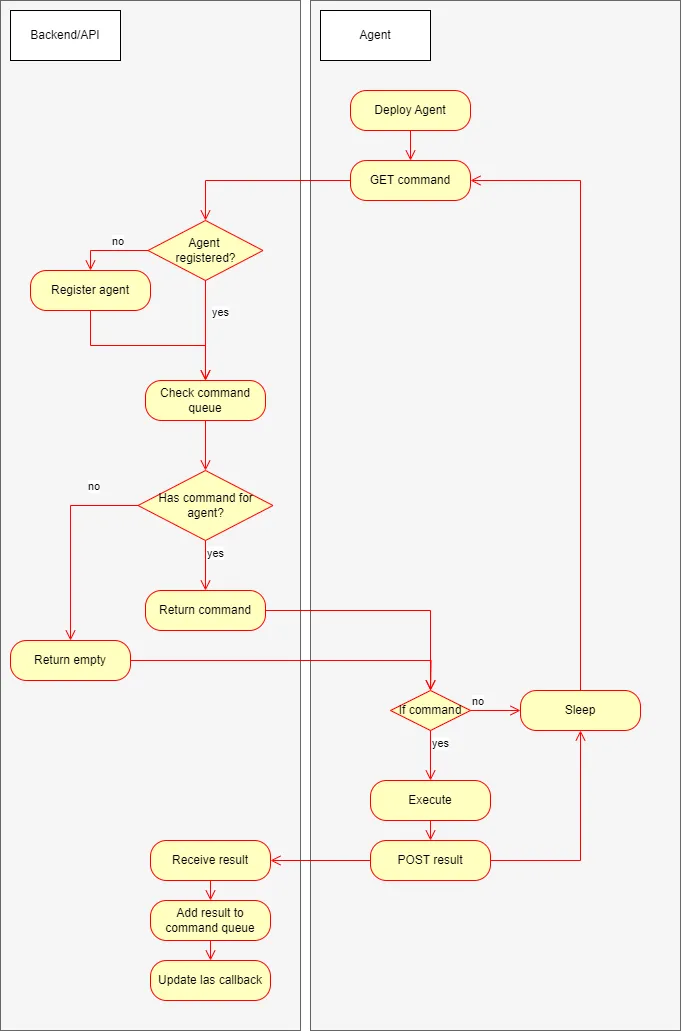
\includegraphics[width=0.8\textwidth]{../includegraphics/diagramm.png} % Ensure path is correct
    \caption{Architectural diagram illustrating the interaction between the Go-based implant, the C2 server, and the React web interface. It shows the agent deployment and communication flow.}
    \label{fig:architecture_diagram}
\end{figure}

\section{C2 Server Implementation (Go \& Gin Gonic)}
\subsection{Project Structure}
The Go-based C2 server, `awesomeProject`, is structured to promote modularity and maintainability. The typical directory layout includes:
\begin{itemize}
    \item \texttt{main.go}: The entry point of the application. It initializes the Gin Gonic router, sets up database connections (utilizing a GORM instance, e.g., `config.DB`), configures routes by calling `routes.SetupRouter()`, and starts the HTTP server. It may also initialize periodic tasks, such as updating inactive implant statuses.
    \item \texttt{config/}: Contains application-wide configurations, most notably the database connection setup (e.g., GORM initialization for \texttt{config.DB}) and potentially JWT secret keys (although the provided code has `jwtSecret` in `controllers/auth.go`).
    \item \texttt{routes/}: Defines all API endpoints. A central \texttt{routes.go} typically contains a `SetupRouter` function that initializes the Gin engine and groups public, implant-facing, and operator-facing (protected) routes, associating them with their respective controller handlers.
    \item \texttt{controllers/}: Houses the Gin handler functions that process incoming HTTP requests, interact with services or database layers, and formulate HTTP responses. Key controller files include:
        \begin{itemize}
            \item \texttt{auth.go}: Manages user authentication, with functions like `Register` and `Login`.
            \item \texttt{implant\_controllers.go}: Contains the core logic for implant interactions, such as `CheckinImplant`, `ImplantClientFetchCommands` (for implants to get tasks), `HandleCommandResult`, `GenerateImplant` (creates a DB record), `DownloadConfiguredImplant` (patches and serves binary), `GetUserImplants` (for dashboard), `SendCommand` (from dashboard to implant), `DashboardGetCommandsForImplant` (for dashboard history), `DeleteImplant`, `HandleLivestreamFrame`, and `GetScreenshotsForImplant`.
            \item \texttt{command\_controller.go}: While much command logic is within \texttt{implant\_controllers.go}, this could be used for more specialized command operations or historical data aggregation if expanded.
        \end{itemize}
    \item \texttt{middleware/}: Contains custom Gin middleware. A crucial piece is \texttt{auth.go} (or similar name), which provides `AuthMiddleware()` for JWT-based authentication, protecting operator-specific API endpoints.
    \item \texttt{models/}: Defines GORM data structures (structs) that map to database tables. These include:
        \begin{itemize}
            \item \texttt{user.go}: The `User` model with username and hashed password.
            \item \texttt{implant.go}: The `Implant` model storing metadata like unique token, status, OS, last seen IP, etc.
            \item \texttt{command.go}: The `Command` model for tasks assigned to implants, including their status and output.
            \item \texttt{screenshot\_info.go}: The `ScreenshotInfo` model for metadata of captured screenshots.
            \item \texttt{fs\_entry.go}: `FileSystemEntry` and `FileSystemListing` structs for file system browsing results.
        \end{itemize}
    \item \texttt{database/}: Provides a data access layer, containing functions that perform CRUD operations and other database queries using the GORM `config.DB` instance. This abstracts complex queries from the controllers (e.g., `GetImplantsByUserID`, `GetPendingCommandsForImplant`, `MarkCommandAsExecuted`, `CreateImplant`).
    \item \texttt{binaries/}: This directory stores pre-compiled base implant executables (e.g., \texttt{base\_client\_windows.exe}, \texttt{base\_client\_linux}). These are used as templates for the `DownloadConfiguredImplant` functionality, where they are patched with specific configurations.
\end{itemize}
This organization separates concerns, making the C2 server's codebase easier to navigate, test, and extend. Implant management, command queuing and execution, and user authentication are handled by dedicated modules interacting primarily through the database.

\subsection{API Endpoint Handling}
The C2 server exposes several RESTful API endpoints for communication with both the implants and the operator's web client. The Gin Gonic framework is utilized for routing and request handling. Below are examples of key endpoint definitions and their corresponding controller logic:

\begin{minted}{go}
// routes/routes.go
// SetupRouter initializes and configures the Gin engine with all application routes.
func SetupRouter() *gin.Engine {
    r := gin.Default() // Creates a Gin router with default middleware (logger, recovery).

    // Public routes for implant communication
    r.POST("/checkin", controllers.CheckinImplant)
    r.GET("/implant-client/:unique_token/commands", controllers.ImplantClientFetchCommands)
    r.POST("/command-result", controllers.HandleCommandResult)
    r.POST("/livestream-frame", controllers.HandleLivestreamFrame)

    // Public routes for user authentication
    r.POST("/register", controllers.Register)
    r.POST("/login", controllers.Login)

    // Protected routes for the Dashboard UI, requiring authentication
    protected := r.Group("/api")
    protected.Use(middleware.AuthMiddleware()) // Applies authentication middleware
    {
        // Implant management and interaction
        protected.GET("/implants", controllers.GetUserImplants)
        protected.POST("/generate-implant", controllers.GenerateImplant) // Creates implant record
        protected.POST("/send-command", controllers.SendCommand)
        protected.GET("/implants/:implant_id/commands", controllers.DashboardGetCommandsForImplant)
        protected.DELETE("/implants/:implant_id", controllers.DeleteImplant)
        // Patches and serves the implant binary
        protected.POST("/implants/:implant_id/download-configured", controllers.DownloadConfiguredImplant)
        protected.GET("/implants/:implant_id/screenshots", controllers.GetScreenshotsForImplant)
    }
    return r
}

// Example: controllers/implant_controller.go (Conceptual snippet for CheckinImplant)
// CheckinImplant handles implant registration and periodic check-ins.
func CheckinImplant(c *gin.Context) {
    var payload struct { // Simplified payload for example
        ImplantID string `json:"implant_id"` // This is unique_token from implant
        PWD       string `json:"pwd"`
    }
    if err := c.ShouldBindJSON(&payload); err != nil {
        c.JSON(http.StatusBadRequest, gin.H{"error": "Invalid payload: " + err.Error()})
        return
    }

    // Logic to update implant status in the database (e.g., using GORM via config.DB):
    // - Find implant by payload.ImplantID (which is its unique_token)
    // - Update 'last_seen' timestamp to time.Now()
    // - Update 'status' to "online"
    // - Update 'ip_address' with c.ClientIP()
    // - Update 'deployed' to true
    
    c.JSON(http.StatusOK, gin.H{"status": "checked_in", "message": "Implant check-in successful"})
}
\end{minted}
Other important controllers include `SendCommand`, which queues a new command for an implant by creating a database record with "pending" status. `HandleCommandResult` updates the command record with the output and "executed" status; it includes special logic for saving screenshot data to files if the output indicates a screenshot. `ImplantClientFetchCommands` allows an implant to retrieve its pending commands. `DownloadConfiguredImplant` is critical for implant delivery, as detailed next.

\subsection{Implant Generation and Configuration}
The C2 server facilitates the generation of customized implant binaries by patching pre-compiled base executables. This process avoids the need for a Go compiler on the C2 server for each implant request. The implant's Go source code itself uses the \texttt{go:embed} directive to include placeholder files which are read at runtime.

The implant source code (which is compiled into the base binaries stored on the C2) contains placeholders like:
\begin{itemize}
    \item \texttt{c2\_address.txt} (embedded content): Contains a placeholder string like \verb|C2_IP_PLACEHOLDER_STRING_PADDING_TO_64_BYTES_XXXXXXXXXXXXXXXXXXXXX|
    \item \texttt{placeholder.txt} (embedded content, for implant ID): Contains a placeholder UUID like \verb|deadbeef-0000-0000-0000-000000000000|
\end{itemize}

When an operator requests a new implant through the web UI:
\begin{enumerate}
    \item The C2 server (via the `GenerateImplant` controller) creates a new implant record in the database, generating a cryptographically secure unique ID (e.g., UUID) for it. The target OS (Windows/Linux) is also stored.
    \item When the operator chooses to download this configured implant (via the `DownloadConfiguredImplant` controller), they provide the C2 server's accessible IP address or domain name (and port) in the request.
    \item The C2 server reads the appropriate pre-compiled base implant binary (e.g., \texttt{binaries/base\_client\_windows.exe} or \texttt{binaries/base\_client\_linux}) from its file system into a byte slice.
    \item The C2 server then performs in-memory binary patching on this byte slice:
        \begin{itemize}
            \item It uses `bytes.LastIndex` to find the byte sequence corresponding to the implant ID placeholder (e.g., \texttt{tokenPlaceholder} variable in the controller). This sequence in the binary is then overwritten with the newly generated unique ID for this implant.
            \item Similarly, it uses `bytes.LastIndex` to find the C2 address placeholder (e.g., \texttt{c2Placeholder} variable). This sequence is overwritten with the C2 server address provided by the operator. The placeholders are padded to a fixed length to ensure the patching is a simple overwrite.
        \end{itemize}
    \item The modified (patched) binary byte slice is then streamed to the operator for download with an appropriate filename (e.g., \texttt{implant\_[unique\_token]\_windows.exe}).
\end{enumerate}
This on-demand patching of pre-compiled executables ensures each implant is uniquely identifiable and configured to communicate with the correct C2 server instance, without requiring on-the-fly compilation on the server. The implant, when run, reads these patched values from its embedded resources.

\subsection{Managing Implant State and Commands}
The C2 server relies on a relational database (interacted with via GORM, using the `config.DB` instance) to persist and manage all implant-related data, including their state, pending commands, and command history.

\begin{description}
    \item[Implant State] Information about each implant is stored in a dedicated table, mapped to the `models.Implant` GORM struct. This includes:
        \begin{itemize}
            \item \texttt{unique\_token}: A unique identifier for the implant, used in API paths and for linking commands.
            \item \texttt{user\_id}: Associates the implant with the operator who generated it.
            \item \texttt{status}: The current operational status (e.g., "new", "online", "offline"). This is updated upon check-ins (`CheckinImplant`), when an implant fetches commands (`ImplantClientFetchCommands`), submits results (`HandleCommandResult`), sends livestream frames (`HandleLivestreamFrame`), or by a periodic server-side task that marks long-unseen implants as "offline" (e.g., `database.UpdateStatusForInactiveImplants`).
            \item \texttt{target\_os}: The operating system of the implant ("windows", "linux").
            \item \texttt{last\_seen}: A timestamp indicating the last time the implant communicated with the C2.
            \item \texttt{ip\_address}: The last known IP address of the implant, updated during check-ins.
            \item \texttt{deployed}: A boolean flag, typically set to `true` after the first successful check-in.
        \end{itemize}

    \item[Commands and Results] Commands intended for implants, along with their execution status and results, are stored in a table mapped to the `models.Command` GORM struct. This includes:
        \begin{itemize}
            \item \texttt{implant\_id}: The \texttt{unique\_token} of the target implant.
            \item \texttt{command}: The actual command string to be executed by the implant.
            \item \texttt{status}: The lifecycle state of the command (e.g., "pending", "executed"). When an operator issues a command via the `SendCommand` controller, a new record is inserted with "pending" status.
            \item \texttt{output}: Stores the textual output or result received from the implant after execution. For screenshots, this field stores a message indicating where the image file was saved on the C2 server (e.g., "Screenshot saved to C2 server at: \texttt{c2\_screenshots/...}").
            \item \texttt{created\_at} and \texttt{updated\_at}: Timestamps for tracking command issuance and completion.
        \end{itemize}
        Implants poll the \texttt{/implant-client/:unique\_token/commands} endpoint (`ImplantClientFetchCommands` controller), which queries the database for "pending" commands for that specific implant using `database.GetPendingCommandsForImplant`. After execution, the implant sends results to \texttt{/command-result} (`HandleCommandResult` controller), which then updates the command's status to "executed" and records the output using `database.MarkCommandAsExecuted`.

    \item[Livestream Data] Livestream frames sent to \texttt{/livestream-frame} (`HandleLivestreamFrame` controller) are saved directly to the C2 server's filesystem under a directory specific to the implant (e.g., \texttt{c2\_screenshots/[implant\_token]/livestream\_frame\_[timestamp].png}).

    \item[Concurrency] The Gin web framework inherently handles concurrent HTTP requests from multiple operators and implants by processing each request in a separate goroutine. GORM, when used with a suitable database system (like PostgreSQL or MySQL), manages concurrent database access. The database connection pool configured with GORM helps in efficiently handling multiple simultaneous database operations. JWTs provide stateless authentication, further simplifying concurrent session management.
\end{description}

\section{Implant Implementation (Go)}
The implants are standalone Go executables designed for cross-platform compatibility and incorporating various functionalities for remote control and data gathering.

\subsection{Core Loop and Communication}
The implant's main operational logic resides in its \texttt{main.go} file. After initial setup, which includes daemonization and self-deletion scheduling, the implant enters a continuous loop.
(Refers to your `implant/main.go` structure)
\begin{minted}{go}
// implant/main.go (simplified conceptual structure)

//go:embed placeholder.txt
var implantIDBytes []byte // Embedded implant ID placeholder

//go:embed c2_address.txt
var c2AddressBytes []byte // Embedded C2 address placeholder

const checkInInterval = 5 * time.Second

var (
    exePath string // Path to the currently running implant executable
    gOriginalLauncherPath string // Path to the initial launcher, passed via env
    // ... other global vars like C2 URLs
)

func main() {
    var err error
    exePath, err = os.Executable() // Path of the CURRENTLY executing file
    if err != nil {
        // Handle error, perhaps log and exit
        os.Exit(1)
    }

    isBackgroundProcess := (os.Getenv(backgroundMarkerEnvVar) == "1")

    if !isBackgroundProcess {
        // This is the initial execution. Relaunch self in background.
        // Call platform-specific relaunchAsDaemonInternal, passing exePath as the
        // original launcher path to be stored in gOriginalLauncherPath by the child.
        // relaunchAsDaemonInternal will copy exePath and run the copy.
        // The original launcher (this process) exits after successful relaunch.
        // ... relaunch logic ...
        os.Exit(0)
    }

    // --- We ARE the background process ---
    os.Unsetenv(backgroundMarkerEnvVar) // Clear marker
    gOriginalLauncherPath = os.Getenv(originalPathEnvVar) // Get original launcher path
    os.Unsetenv(originalPathEnvVar) // Clear for security

    if !initializeConfig() { // Parses embedded C2_ADDRESS & IMPLANT_ID
        os.Exit(1) // Exit if config is invalid
    }

    // Schedule self-deletion in a separate goroutine.
    // This targets both the current running implant (exePath) and the
    // original launcher (gOriginalLauncherPath).
    if doSelfDelete != nil {
        go func() {
            time.Sleep(2 * time.Second) // Brief delay for implant startup
            doSelfDelete(exePath, gOriginalLauncherPath)
        }()
    }

    // Main operational loop
    for {
        checkIn() // Send heartbeat and PWD to C2
        // Pass current exePath (of this backgrounded process) AND the original launcher's path
        fetchAndExecuteCommands(exePath, gOriginalLauncherPath)
        time.Sleep(checkInInterval)
    }
}

// initializeConfig populates C2 URLs from embedded c2AddressBytes
// and verifies implantIDBytes.
func initializeConfig() bool { /* ... */ return true }

// checkIn sends a POST request to the C2 server's /checkin endpoint.
func checkIn() { /* ... */ }

// fetchAndExecuteCommands retrieves commands from the C2 server and processes them.
func fetchAndExecuteCommands(currentImplantExePath string, originalLauncherPath string) {
    // ... HTTP GET to C2's command URL for this implant ...
    // ... JSON unmarshal commands from response ...

    // For each command received:
    // Example command parsing:
    // if strings.HasPrefix(trimmedCmdStr, "fs_browse ") { listDirectory(...) }
    // else if trimmedCmdStr == "screenshot" { takeScreenshotAndSend() }
    // else if trimmedCmdStr == "livestream_start" { startLivestreamGoroutine() }
    // else if trimmedCmdStr == "self_destruct" {
    //     sendOutput(cmdToExec.ID, "Self-destruct initiated...")
    //     if doSelfDelete != nil {
    //         // Initiate deletion of current implant and original launcher
    //         doSelfDelete(currentImplantExePath, originalLauncherPath)
    //     }
    //     os.Exit(0) // Terminate implant to allow file deletion
    // }
    // else { /* Execute general shell command using os/exec */ }
    // ... After execution, call sendOutput() with results ...
}

// sendOutput sends the result of a command back to the C2 server.
func sendOutput(cmdID int, output string) { /* ... */ }

// doSelfDelete is a platform-specific function pointer.
var doSelfDelete func(selfExePath string, originalLauncherPath string)

// (Other platform-specific function pointers like takeScreenshot, setOSSpecificAttrs)
\end{minted}

\subsection{Daemonization Techniques}
To operate stealthily, implants employ platform-specific techniques to run as background processes without direct user interaction or visible console windows. The initial executable (launcher) is responsible for creating a detached, hidden copy of itself.

\subsubsection{Windows (\texttt{relaunch\_windows.go})}
The \texttt{relaunchDaemonWindows} function in \texttt{relaunch\_windows.go} handles daemonization on Windows systems:
\begin{itemize}
    \item The currently running executable's path (\texttt{currentExePath}, which is the initial launcher) is identified.
    \item This executable is copied to a new, often innocuously named file (e.g., \texttt{audiosrvhost\_[timestamp]\_[random].exe}) within the user's temporary directory (\texttt{os.TempDir()}).
    \item An \texttt{exec.Command} is prepared to run this newly copied executable.
    \item Crucially, two environment variables are set for the new process:
        \begin{itemize}
            \item \texttt{IMPLANT\_IS\_BACKGROUND\_XYZ123=1}: A marker indicating this new process is the daemonized instance.
            \item \texttt{IMPLANT\_ORIG\_LAUNCHER\_PATH\_XYZ789=[path\_to\_currentExePath]}: Stores the path of the original launcher, which the daemonized implant will need for self-deletion purposes.
        \end{itemize}
    \item The \texttt{SysProcAttr} of the command is configured with:
        \begin{itemize}
            \item \texttt{HideWindow: true}
            \item \texttt{CreationFlags: 0x08000000 \textbar \ 0x00000008} (CREATE\_NO\_WINDOW \textbar \ DETACHED\_PROCESS). These flags ensure the new process runs without a console window and is detached from the parent's console session.
        \end{itemize}
    \item The new process is started using \texttt{cmd.Start()}.
    \item The parent process (the initial launcher) then calls \texttt{cmd.Process.Release()} to detach from the child process, allowing the child to continue running independently.
    \item Finally, the initial launcher process (\texttt{currentExePath}) exits (\texttt{os.Exit(0)}). The backgrounded copy, upon starting, checks for the \texttt{IMPLANT\_IS\_BACKGROUND\_XYZ123} environment variable, retrieves the original launcher's path from \texttt{IMPLANT\_ORIG\_LAUNCHER\_PATH\_XYZ789}, and proceeds with its C2 operations.
\end{itemize}

\subsubsection{Linux (\texttt{platform\_linux.go})}
On Linux, daemonization is achieved by the \texttt{linuxRelaunchAsDaemon} function in \texttt{platform\_linux.go}:
\begin{itemize}
    \item The path of the executable to be daemonized (\texttt{originalLauncherExecutablePath}, which is the initial launcher) is taken as input.
    \item This executable is copied to a temporary file with a randomized name (e.g., \texttt{/tmp/implant\_[randomhex]}) and made executable.
    \item An \texttt{exec.Command} is prepared to run this temporary executable. The first argument to the command (\texttt{argv[0]}) is set to a desired spoofed name (e.g., \texttt{[kthreadd]}) to masquerade the process in listings.
    \item Similar to Windows, environment variables \texttt{IMPLANT\_IS\_BACKGROUND\_XYZ123=1} and \texttt{IMPLANT\_ORIG\_LAUNCHER\_PATH\_XYZ789=[originalLauncherExecutablePath]} are set for the new process.
    \item The \texttt{SysProcAttr} of the command is configured with \texttt{Setsid: true}. This creates a new session and detaches the process from the controlling terminal, making it a daemon.
    \item The new process is started using \texttt{cmd.Start()}.
    \item Immediately after successful start, the temporary executable file (\texttt{/tmp/implant\_[randomhex]}) is deleted from the filesystem using \texttt{os.Remove()}. This results in the daemonized process running from an unlinked file, a common "fileless" execution characteristic for the copied instance.
    \item The initial launcher process (\texttt{originalLauncherExecutablePath}) then exits (\texttt{os.Exit(0)}). The daemonized implant proceeds as described for the Windows case.
\end{itemize}
Additionally, the Linux implant attempts to further obfuscate its presence by calling \texttt{prctl(PR\_SET\_NAME, ...)} via CGo (in \texttt{proc\_rename\_linux.go}) to change its kernel thread name, although this name is typically truncated to 15 characters.

\begin{figure}[H]
    \centering
    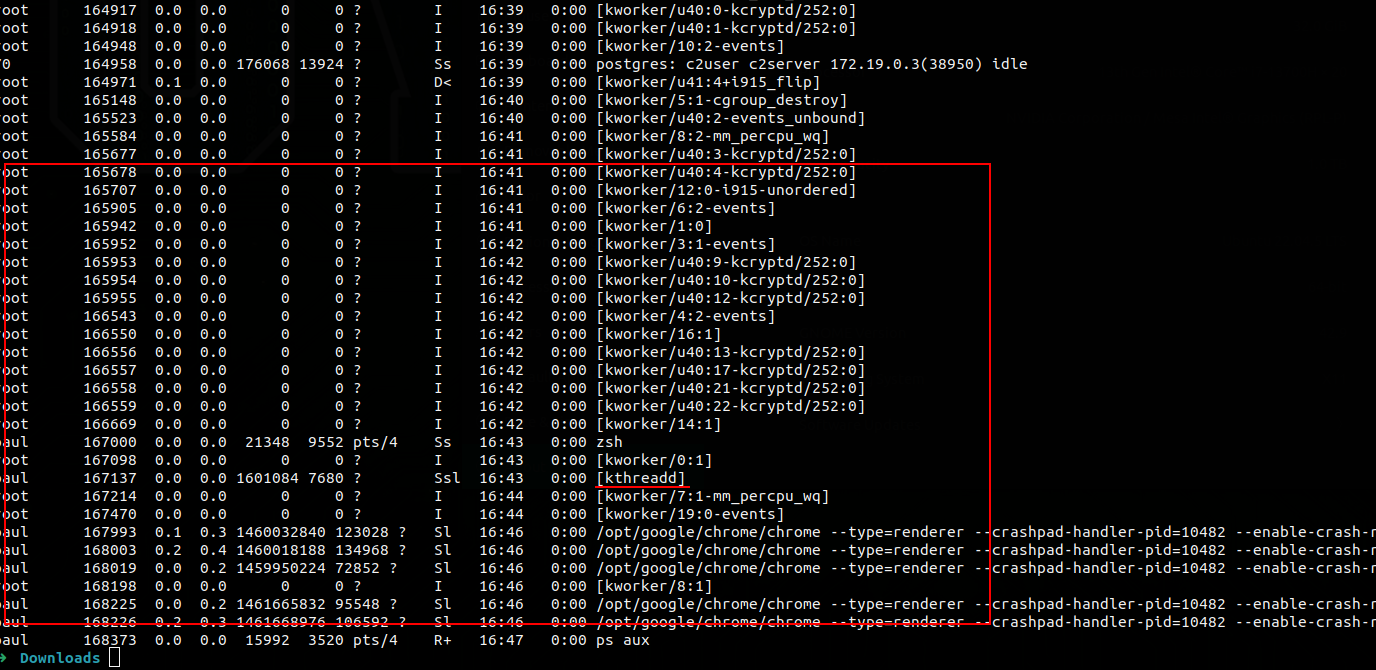
\includegraphics[width=0.8\textwidth]{../screenshots/linux_process_list.png} % Ensure path is correct
    \caption{A screenshot from a Linux system showing the implant process masquerading with a common kernel thread name, `[kthreadd]` (actual name may vary based on implant configuration).}
    \label{fig:linux_process_masquerade}
\end{figure}

\subsection{Self-Deletion Mechanisms}
To minimize forensic artifacts, implants are designed to delete both the initial launcher executable and their own currently running executable file (the daemonized copy) upon receiving a \texttt{self\_destruct} command or potentially as a final cleanup step.

\subsubsection{Windows (\texttt{exec\_attrs\_windows.go})}
The \texttt{doSelfDeleteWindows} function orchestrates self-deletion on Windows:
\begin{description}
    \item[Deleting the Original Launcher] If an \texttt{originalLauncherPath} is provided (and is different from the current implant's path), the \texttt{deleteFileViaBatch} function is called. This function:
        \begin{itemize}
            \item Creates a temporary batch script (e.g., \texttt{del\_file\_proc[PID]\_time[NANO].bat}) in \texttt{os.TempDir()}.
            \item The batch script contains commands to forcefully delete the specified \texttt{originalLauncherPath} and then delete the batch script itself.
            \item This batch script is executed as a new, detached, and hidden process (\texttt{cmd.exe /C [batch\_file\_path]} with \texttt{CREATE\_NO\_WINDOW | DETACHED\_PROCESS}). The parent Go process does not wait for its completion.
        \end{itemize}
    \item[Marking the Current Implant for Deletion] The \texttt{markFileForDeleteOnCloseAndPosixSemantics} function is called with the path to the currently running implant executable (\texttt{selfExePath}). This function:
        \begin{itemize}
            \item Opens a handle to \texttt{selfExePath} with \texttt{DELETE} access and \texttt{FILE\_SHARE\_DELETE}.
            \item Calls the Windows API \texttt{SetFileInformationByHandle} with the class \texttt{FileDispositionInformationEx} (value 64) and a structure containing the flags \texttt{FILE\_DISPOSITION\_FLAG\_DELETE | FILE\_DISPOSITION\_FLAG\_POSIX\_SEMANTICS}.
            \item This marks the file such that it will be deleted by the operating system once the last handle to it is closed (i.e., when the implant process exits). The POSIX semantics flag also helps prevent new handles from being opened to the file.
        \end{itemize}
\end{description}
After initiating these deletion mechanisms, if the implant receives a \texttt{self\_destruct} command, it will call \texttt{os.Exit(0)} to allow the file system operations to complete.

\subsubsection{Linux (\texttt{platform\_linux.go})}
On Linux, the \texttt{linuxScheduleSelfDeleteGrandchild} function handles deletion:
\begin{description}
    \item[Deleting the Original Launcher] If \texttt{originalLauncherPath} is valid and different from \texttt{selfExePath}, a shell command is constructed: \verb|sleep 1 && rm -f "[quoted_originalLauncherPath]"|.
        \begin{itemize}
            \item This command is executed using \texttt{exec.Command("sh", "-c", ...)}.
            \item \texttt{SysProcAttr} is set with \texttt{Setsid: true} to detach the deletion process.
            \item The command is started with \texttt{cmd.Start()}, and a separate goroutine calls \texttt{cmd.Wait()} to reap the child process and prevent it from becoming a zombie.
        \end{itemize}
    \item[Deleting the Current Implant Executable] A similar shell command is constructed for \texttt{selfExePath}: \verb|sleep 3 && rm -f "[quoted_selfExePath]"|. This also uses a detached process with \texttt{Setsid: true} and is reaped by a goroutine. The slightly longer sleep (3 seconds) is to give the implant a moment to fully exit if the self-destruct command also triggers \texttt{os.Exit(0)}.
\end{description}
Upon a \texttt{self\_destruct} command, the implant calls \texttt{os.Exit(0)}, allowing these scheduled \texttt{rm} commands to delete the unlinked (for the daemonized copy) and original launcher files.

\subsection{Screenshot and Livestreaming}
Implants can capture screenshots of the host's desktop and stream them to the C2 server.

\subsubsection{Screenshot Capabilities (\texttt{screenshot\_linux.go}, \texttt{exec\_attrs\_windows.go})}
The \texttt{takeScreenshot} function pointer is assigned a platform-specific implementation:
\begin{description}
    \item[Windows] Utilizes the \texttt{github.com/kbinani/screenshot} package. It captures the primary display's bounds using \texttt{screenshot.GetDisplayBounds(0)} and then captures the rectangle with \texttt{screenshot.CaptureRect()}. The resulting image is encoded to PNG format and then Base64 encoded for transmission.
    \item[Linux] The \texttt{linuxTakeScreenshot} function attempts a series of external screenshot utilities commonly found on Linux systems, in order of preference (e.g., \texttt{grim} for Wayland, \texttt{maim} for X11, \texttt{import} from ImageMagick, \texttt{scrot}).
        \begin{itemize}
            \item For each utility, it first checks if the command exists using \texttt{exec.LookPath()}.
            \item It then tries to execute the utility with arguments that pipe the PNG output directly to standard output. If successful, this output is captured.
            \item If piping to stdout fails or is not supported by the utility, it attempts to save the screenshot to a temporary PNG file. This file is then read.
            \item The captured image data (from stdout or the temp file) is Base64 encoded.
            \item If all attempts fail, an error is returned.
        \end{itemize}
\end{description}
The Base64 encoded screenshot data is prefixed with \texttt{"screenshot\_data:"} and sent to the C2 server.

\subsubsection{Livestreaming Logic (\texttt{implant/main.go})}
Desktop livestreaming is initiated by the \texttt{livestream\_start} command from the C2:
\begin{itemize}
    \item Sets a flag \texttt{isLivestreamActive} to true.
    \item Creates a \texttt{stopLivestreamChan} channel.
    \item Launches the \texttt{runLivestream} function in a new goroutine.
    \item \texttt{runLivestream} uses a \texttt{time.NewTicker} (typically set for 1-second intervals, i.e., 1 FPS).
    \item On each tick, it calls the platform-specific \texttt{takeScreenshot()} function.
    \item The Base64 encoded frame data is then sent to the C2 server's \texttt{/livestream-frame} endpoint via an HTTP POST request in a \texttt{LivestreamFramePayload}.
    \item The livestream continues until the \texttt{livestream\_stop} command is received, which closes the \texttt{stopLivestreamChan}, causing the \texttt{runLivestream} goroutine to terminate.
\end{itemize}

\subsection{File System Interaction (\texttt{fs\_utils.go})}
Implants provide capabilities to browse the remote file system and download files. These are primarily handled by functions in \texttt{fs\_utils.go}.
\begin{description}
    \item[\texttt{listDirectory(path string)}]
        \begin{itemize}
            \item Takes a directory path as input.
            \item Uses \texttt{os.ReadDir} to get a list of \texttt{os.DirEntry} items.
            \item For each entry, it calls \texttt{entry.Info()} to get \texttt{os.FileInfo}, from which it extracts the \texttt{Name}, \texttt{IsDir}, \texttt{Size}, \texttt{ModTime}, and \texttt{Mode().String()} (permissions).
            \item Constructs a \texttt{FileSystemListing} struct containing a slice of \texttt{FileSystemEntry} structs and sends this JSON-marshaled data to the C2.
        \end{itemize}
    \item[\texttt{listRoots()}]
        \begin{itemize}
            \item Provides a list of root directories.
            \item On Windows, it iterates from drive 'A' to 'Z', checking for existence with \texttt{os.Stat(drive + ":\\")}.
            \item On Linux and other Unix-like systems, it typically lists the root directory \texttt{"/"}.
            \item Returns a \texttt{FileSystemListing} similar to \texttt{listDirectory}.
        \end{itemize}
    \item[File Download (handled in \texttt{fetchAndExecuteCommands})]
        \begin{itemize}
            \item Triggered by an \texttt{fs\_download} command specifying a file path.
            \item Uses \texttt{os.ReadFile} to read the entire file content into a byte slice.
            \item The byte slice is then Base64 encoded.
            \item The encoded data is prefixed with \texttt{"file\_data\_b64:"} and sent to the C2 server as the command's output.
        \end{itemize}
\end{description}
The implant also supports the \texttt{cd} command, which uses \texttt{os.Chdir} to change the implant's current working directory. The updated PWD is reflected in subsequent check-ins.

\section{Web Client Implementation (React)}
The web client is a Single Page Application (SPA) built with React, providing the operator with an interface to interact with the C2 server and manage implants.

\subsection{Project Structure}
The React application's \texttt{src} directory is organized to separate concerns, typically including:
\begin{itemize}
    \item \texttt{App.js}: The root component of the application, responsible for setting up client-side routing (likely using `react-router-dom`, as evidenced by `useNavigate` and `Link` imports in components) and rendering top-level layout.
    \item \texttt{index.js}: The main entry point that renders the \texttt{App} component into the DOM.
    \item \texttt{components/}: This directory houses a collection of reusable UI components and potentially page-level views. Based on the provided code, key components include:
        \begin{itemize}
            \item \texttt{AuthForm.js}: Handles user registration and login forms.
            \item \texttt{Dashboard.js}: Serves as the main operational view after login. It displays the list of implants, provides controls for implant generation, download, deletion, and access to interactive features like the terminal, file explorer, and screenshot/livestream viewers. It also manages global UI elements like notifications and modals.
            \item \texttt{Terminal.js}: An interactive pseudo-terminal for sending commands to a selected implant and viewing output.
            \item \texttt{FileSystemExplorer.js}: A component for browsing the file system of a selected implant.
            \item \texttt{ScreenshotViewer.js}: A modal component for displaying individual screenshots in a gallery format or a live desktop stream.
            \item \texttt{DownloadOptionsModal.js}: A modal dialog for specifying the C2 server IP when downloading a configured implant.
            \item \texttt{GenerateImplantOSModal.js}: A modal for selecting the target OS when creating a new implant record.
            \item (Other modals like `DeleteConfirmationModal` are defined as sub-components or directly within `Dashboard.js`).
        \end{itemize}
    \item \texttt{services/} or \texttt{api/}: While not explicitly shown as a separate directory in the provided snippets, API calls to the C2 backend are made using the browser's `fetch` API directly within components (e.g., in `Dashboard.js`, `Terminal.js`, `AuthForm.js`). In larger applications, this logic might be abstracted into dedicated service modules.
    \item \texttt{hooks/}: Custom React hooks for encapsulating reusable stateful logic or side effects are a common pattern, although no specific custom hooks are detailed in the provided code.
    \item \texttt{context/} or \texttt{store/}: Global state management beyond component-level state and prop drilling is not explicitly demonstrated. The application appears to rely on:
        \begin{itemize}
            \item Local component state managed by `useState` and `useRef`.
            \item Passing state and callbacks down through props (prop drilling), for example, `displayNotification` and `openScreenshotViewer` functions from `Dashboard.js`.
            \item `localStorage` is utilized to persist the JWT authentication token and the operator's preferred default C2 IP address across sessions.
        \end{itemize}
        For more complex state interdependencies, React Context API or libraries like Redux/Zustand could be integrated.
    \item CSS files (\texttt{App.css}, \texttt{index.css}, \texttt{styles.css}): Standard CSS files for styling. The use of class names like `flex`, `bg-gray-900`, `rounded-lg` suggests the adoption of a utility-first CSS framework like Tailwind CSS.
\end{itemize}

\subsection{Key Components}
The React frontend is composed of several key components that enable operator interaction:
\begin{description}
    \item[\\texttt{Dashboard.js}] This is the central hub for operators. It fetches and displays a list of active and inactive implants from the C2 server\'s \\verb|/api/implants| endpoint, showing details like ID (Token), OS, Status, Last Seen, and IP Address. From here, operators can:
        \\begin{itemize}
            \\item Initiate the generation of new implant records via \\texttt{GenerateImplantOSModal.js}.
            \\item Configure and download implant binaries via \\texttt{DownloadOptionsModal.js}.
            \\item Delete implants (with confirmation).
            \\item Open an interactive \\texttt{Terminal.js} for a selected implant.
            \\item Launch \\texttt{ScreenshotViewer.js} to view collected screenshots or start a live desktop stream.
            \\item Open \\texttt{FileSystemExplorer.js} for a selected implant.
            \\item Manage a global C2 IP setting for implant downloads.
            \\item It also handles displaying system-wide notifications.
        \\end{itemize}

    \begin{figure}[H]
        \\centering
        \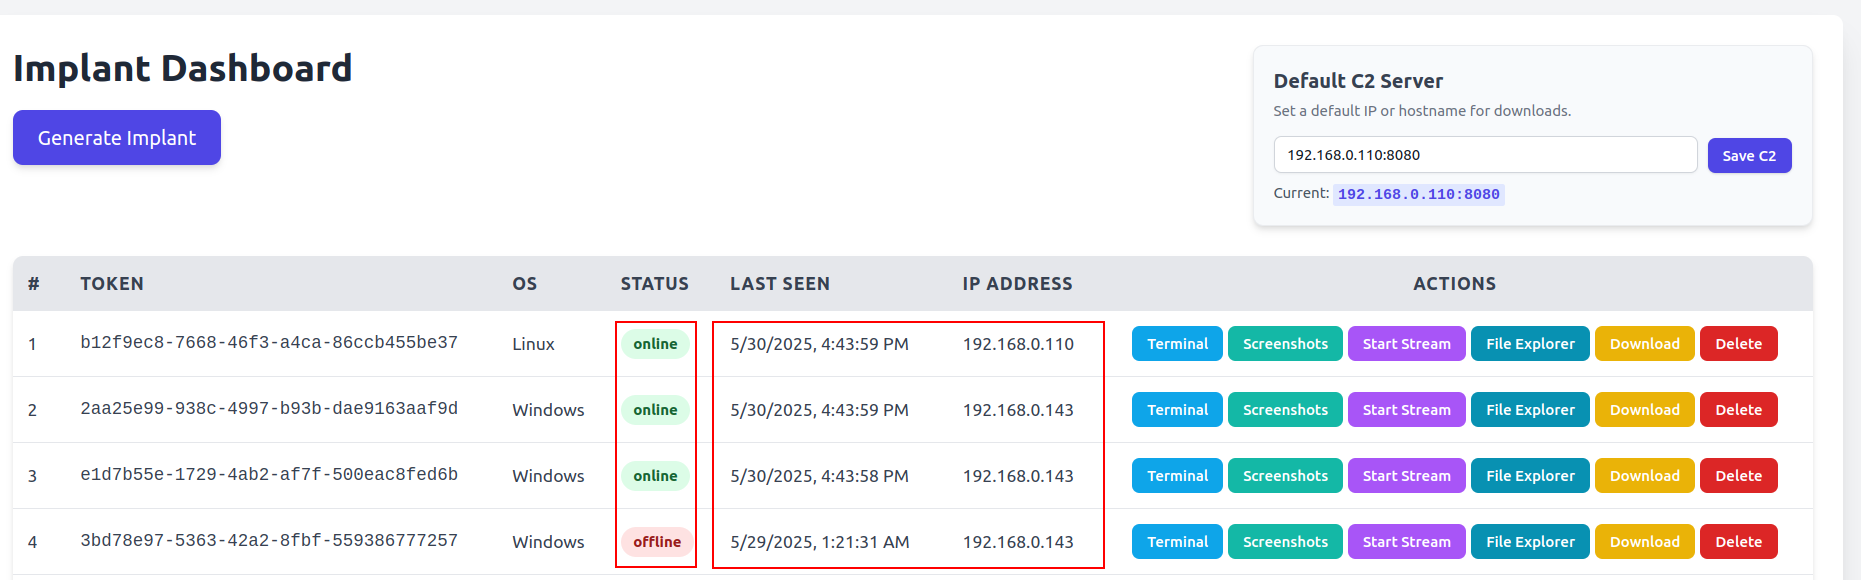
\includegraphics[width=0.8\\textwidth]{../screenshots/c2_dashboard.png} % Ensure path is correct
        \\caption{The C2 dashboard interface, showcasing the list of managed implants, their status, and available actions.}
        \\label{fig:c2_dashboard}
    \\end{figure}

    \\item[\\texttt{Terminal.js}] Provides an interactive pseudo-terminal interface for a specific implant.
        \\begin{itemize}
            \\item An input field allows the operator to type commands.
            \\item On submission, the command is sent to the C2 server via a POST request to \\verb|/api/send-command|, along with the selected implant\'s ID.
            \\item It periodically fetches new and updated command statuses/outputs for the active implant from the C2 server (e.g., \\verb|/api/implants/:implant_id/commands|) and displays the command history and output.
            \\item If a command output indicates a saved screenshot, it provides a button to open it in the \\texttt{ScreenshotViewer.js}.
        \\end{itemize}

    \begin{figure}[H]
        \\centering
        \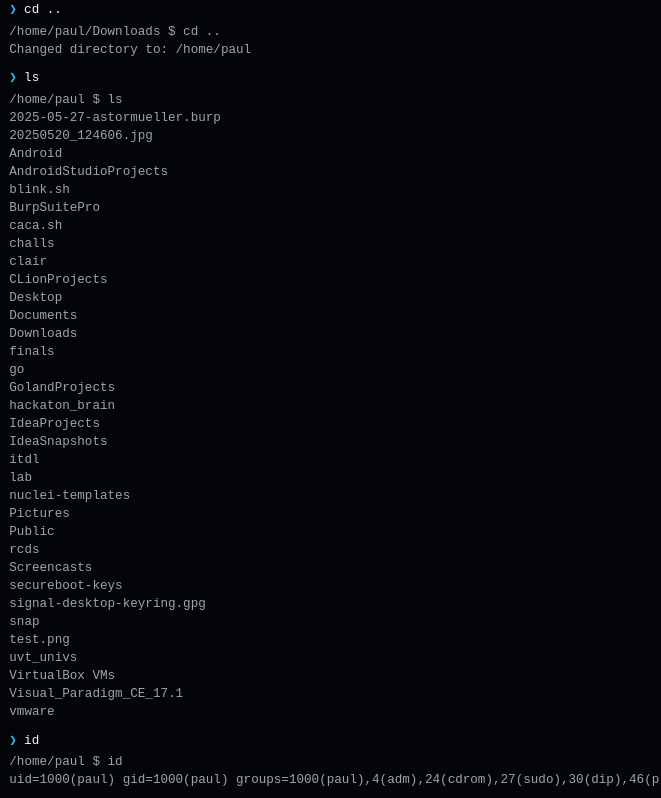
\includegraphics[width=0.8\\textwidth]{../screenshots/terminal.png} % Ensure path is correct
        \\caption{The interactive terminal within the C2 web interface, allowing operators to send commands to and receive output from an implant.}
        \\label{fig:c2_terminal}
    \\end{figure}

    \\item[\\texttt{FileSystemExplorer.js}] Renders a file and directory listing received from an implant (after an \\texttt{fs\\_browse} command). It allows:
        \\begin{itemize}
            \\item Navigation into subdirectories (by issuing new \texttt{fs\_browse} commands via `cd` equivalent logic or by clicking on directory entries which changes the `currentPath` state, triggering a new browse command).
            \\item Navigation up to parent directories.
            \\item Triggering file downloads by sending \texttt{fs\_download} commands for selected files.
            \\item It polls for command results similarly to the terminal.
        \\end{itemize}
    \\item[\\texttt{ScreenshotViewer.js}] A modal component responsible for displaying images.
        \\begin{itemize}
            \\item In 'gallery' mode, it displays individual screenshots fetched from the C2 server (e.g., from URLs like \\texttt{/c2\\_screenshots/:implant\\_id/:filename.png} which are served statically by the C2, paths obtained via \\verb|/api/implants/:implant_id/screenshots|). It provides navigation controls (next/previous, slideshow).
            \\item In 'livestream' mode, it continuously updates an \\texttt{<img>} tag with the latest frame fetched from the C2 (image paths are polled).

            \begin{figure}[H]
                \\centering
                \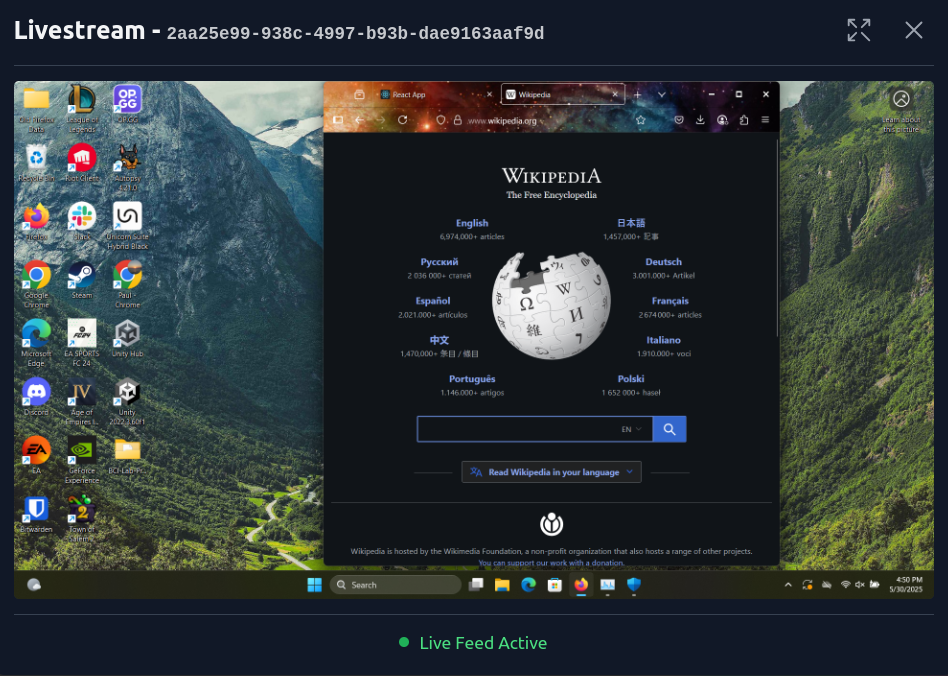
\includegraphics[width=0.8\\textwidth]{../screenshots/livestream.png} % Ensure path is correct
                \\caption{Example of the livestream feature, displaying a real-time screen capture from a compromised implant.}
                \\label{fig:livestream_example}
            \\end{figure}

            \\item Supports a fullscreen mode for better viewing.
            \\item When closed in 'livestream' mode, it can trigger a \\texttt{livestream\\_stop} command to be sent to the implant.
        \\end{itemize}
    \\item[Authentication Components (\\texttt{AuthForm.js})] Handles user registration and login.
        \\begin{itemize}
            \\item Makes POST requests to the C2 server's \verb|/register| and \verb|/login| endpoints.
            \\item Upon successful authentication, it stores the received JWT in `localStorage`.
            \\item Navigates the user to the \texttt{/dashboard}.
        \\end{itemize}
    \\item[Modal Components (\\texttt{GenerateImplantOSModal.js}, \texttt{DownloadOptionsModal.js})]
        \\begin{itemize}
            \\item \texttt{GenerateImplantOSModal.js}: A form allowing the operator to select the target OS (Windows/Linux) for a new implant. Triggers an API call to \verb|/api/generate-implant| to create the implant record in the C2 database.
            \\item \texttt{DownloadOptionsModal.js}: A form that appears when downloading a configured implant. It prompts the operator for the C2 server's IP address (pre-filled with a global default if set) which will be embedded into the implant binary. Triggers a POST request to \verb|/api/implants/:implant_id/download-configured|.
        \\end{itemize}
\end{description}

(Below is a conceptual React snippet for a simplified terminal input component)
\begin{minted}{js}
// Example: Simplified TerminalInput.js component (part of Terminal.js)
import React, { useState } from 'react';
// Assume 'apiService.sendCommandToImplant' is a function that POSTs to the C2.

function TerminalInput({ selectedImplantId, onCommandSent }) {
    const [command, setCommand] = useState('');
    const [isLoading, setIsLoading] = useState(false);


    const handleSubmit = async (event) => {
        event.preventDefault();
        if (!command.trim() || !selectedImplantId || isLoading) return;
        setIsLoading(true);

        try {
            // Example API call structure within Terminal.js:
            // const token = localStorage.getItem("token");
            // const res = await fetch("/api/send-command", {
            //   method: "POST",
            //   headers: { "Content-Type": "application/json", Authorization: `Bearer ${token}` },
            //   body: JSON.stringify({ implant_id: selectedImplantId, command: command }),
            // });
            // if (!res.ok) { /* handle error */ }
            // Optimistic UI update or rely on poller in Terminal.js
            console.log(`Sending command: ${command} to ${selectedImplantId}`);


            setCommand(''); // Clear input field
            if (onCommandSent) { // Callback might trigger immediate fetch or rely on existing poller
                onCommandSent();
            }
        } catch (error) {
            console.error("Error sending command:", error);
            // Handle error (e.g., display a notification to the user)
        } finally {
            setIsLoading(false);
        }
    };

    return (
        <form onSubmit={handleSubmit} className="flex items-center p-2">
            <span className="text-blue-400 mr-2">{">"}</span>
            <input
                type="text"
                value={command}
                onChange={(e) => setCommand(e.target.value)}
                placeholder="Enter command..."
                disabled={!selectedImplantId || isLoading}
                className="flex-grow bg-transparent focus:outline-none"
                autoFocus
            />
            <button type="submit" disabled={!selectedImplantId || !command.trim() || isLoading}
                    className="bg-blue-500 text-white px-3 py-1 rounded ml-2 hover:bg-blue-600 disabled:opacity-50">
                {isLoading ? "Sending..." : "Send"}
            </button>
        </form>
    );
}

export default TerminalInput;
\end{minted}

\subsection{State Management and API Interaction}
\begin{description}
    \item[State Management]
    The React application primarily employs component-level state management using React's built-in hooks:
    \begin{itemize}
        \item \texttt{useState}: Used extensively for managing local component data, such as input field values, lists of items (e.g., implants, commands, file entries), modal visibility, loading indicators, and error messages.
        \item \texttt{useEffect}: Manages side effects, including fetching initial data when a component mounts, setting up and tearing down intervals for polling.
        \item \texttt{useRef}: Utilized for accessing underlying DOM elements (e.g., `containerRef` in `Terminal.js` for scrolling, `viewerContentRef` in `ScreenshotViewer.js` for fullscreen) and for storing mutable values that do not trigger re-renders across the component lifecycle (e.g., `polling.current` flag, interval IDs).
    \end{itemize}
    For cross-component state or actions, the application relies on:
    \begin{description}
        \item[Prop Drilling] Callbacks and state values are passed down from parent components to children (e.g., `displayNotification` function and `openScreenshotViewer` function are passed from `Dashboard.js` to child components like `Terminal.js` and `FileSystemExplorer.js`).
        \item[\texttt{localStorage}] Used for persisting data across browser sessions, specifically the JWT authentication token (`token`) obtained after login and a user-configurable global C2 IP address (`dashboardGlobalC2IP`) used as a default for implant downloads.
    \end{description}
    While no global state management libraries like Redux or Zustand, or React's Context API, are explicitly shown in the provided snippets for application-wide state, these could be integrated if the complexity of state sharing grows.

    \item[API Interaction]
    Communication with the C2 server's RESTful API is handled using the browser's native \texttt{fetch} API:
    \begin{itemize}
        \item API calls are typically encapsulated within asynchronous functions (`async/await`) inside React components, often triggered by user interactions (e.g., button clicks) or by `useEffect` hooks (e.g., for initial data loading or polling).
        \item For requests to protected API endpoints (those under the `/api` group), the JWT stored in `localStorage` is retrieved and included in the `Authorization` header as a Bearer token (e.g., `headers: \{ 'Authorization': \`Bearer \$\{token\}\` \}`).
        \item Request bodies for `POST` or `PUT` methods are usually JSON, prepared using `JSON.stringify()`.
        \item Server responses are typically expected in JSON format and are parsed using `response.json()`.
        \item \textbf{Polling:} For real-time updates in the terminal, screenshot viewer (livestream), and file explorer, `setInterval` is used within `useEffect` hooks to periodically call relevant API endpoints. These intervals are cleared in the `useEffect` cleanup function to prevent memory leaks and unnecessary calls when the component unmounts or the polling condition changes. The `Dashboard.js` component also checks `document.hidden` to pause screenshot polling when the browser tab is not active.
    \end{itemize}

    \item[Error Handling and Loading States]
    \begin{description}
        \item[Error Handling] API calls made with `fetch` are wrapped in `try...catch` blocks to handle network errors or exceptions during the request/response cycle. Non-`2xx` HTTP status codes are checked (e.g., `if (!response.ok)`), and error messages are often parsed from the JSON response body. Errors are communicated to the user via a centralized notification system (the `Notification` component in `Dashboard.js`, triggered by the `displayNotification` function) or through component-specific error messages displayed in the UI.
        \item[Loading States] Boolean state variables (e.g., `loading` in `Terminal.js`, `isInitiallyLoading` and `isManuallyRefreshing` in `FileSystemExplorer.js`, `isLoadingInitial` in `ScreenshotViewer.js`) are used to track the asynchronous nature of API calls. These states control UI elements by:
            \begin{itemize}
                \item Disabling buttons or input fields during an operation to prevent duplicate submissions.
                \item Displaying loading indicators like spinners or textual messages (e.g., "Loading...", "Sending...").
                \item Conditionally rendering parts of the UI based on whether data is available or an operation is in progress.
            \end{itemize}
    \end{description}
\end{description}

\section{Challenges Encountered and Solutions}
Throughout the development of this C2 framework, several technical challenges were encountered:
\begin{itemize}
    \item Cross-Platform Nuances in Implants: Ensuring consistent behavior for daemonization, self-deletion, and screenshotting across Windows and Linux required careful use of Go's build tags (e.g., \\texttt{//go:build windows}) and platform-specific API calls or external utilities. For example, Windows file deletion required a combination of marking files for delete-on-close and using detached batch scripts for locked files, while Linux relied on detached \\texttt{rm} commands.
    \item Reliable Self-Deletion: Deleting an executable while it is running, or deleting its original launcher, is inherently tricky due to file locking by the OS. The solutions involved detached processes (batch scripts on Windows, \\texttt{sh -c} on Linux) and OS-specific APIs like \\texttt{SetFileInformationByHandle} on Windows.
    \item Process Hiding and Masquerading on Linux: While changing \\texttt{argv[0]} during the \\texttt{execve} syscall (achieved by setting \\texttt{cmd.Args[0]} in Go before \\texttt{cmd.Start()} for the daemonized copy) is effective for altering how the process appears in tools like \texttt{ps}, the \texttt{prctl(PR\\_SET\\_NAME)} call has limitations (e.g., 15-character limit, only affects thread name). A combination provides better, though not perfect, obfuscation.
    \item React State Management for Real-time Updates: Efficiently updating the UI for features like the livestreaming desktop view or the interactive terminal (which requires polling for new command outputs) without causing performance degradation or excessive re-renders required careful state management (primarily `useState`, `useEffect`), memoization where necessary (e.g., \\texttt{React.memo}, \\texttt{useMemo}, \\texttt{useCallback}, though not explicitly detailed in provided code, these are common optimizations), and ensuring polling intervals are managed correctly (cleared on unmount, paused when tab is hidden).
    \item Implant Configuration and Delivery: The method of patching pre-compiled base binaries with C2 addresses and implant IDs is efficient as it avoids needing a Go compiler on the C2 server. However, the placeholder strings and the patched information are stored as plain text within the binary. This means if an implant binary is captured, the C2 address can be easily extracted. More advanced C2s might use encrypted configuration blocks or staged loading to better protect this information. The current approach trades some operational security for simplicity in generation and deployment.
    \item Locating and Patching Embedded Placeholders in Pre-compiled Binaries: The implant generation relies on finding specific placeholder byte sequences within pre-compiled base binaries to patch in the unique implant ID and C2 server address. Ensuring these placeholders are unique enough not to appear elsewhere in the binary by chance, are of a fixed and known size, and that the patching process correctly overwrites them without corrupting the executable requires careful management of the base binary's compilation (ensuring placeholders exist) and the patching logic on the C2 server (using `bytes.LastIndex`). The implant then uses `go:embed` to access these (now patched) values from its embedded resources at runtime.
    \item Handling Concurrent Operations on the C2 Server: While Gin handles concurrent HTTP requests, ensuring that database operations are performed safely and without race conditions required reliance on GORM's capabilities and the underlying database's concurrency control mechanisms. For instance, updating implant 'last seen' times or command statuses from multiple concurrent implant check-ins needs to be handled correctly by the database.
    \item Robust Screenshot and Livestream File Management: Saving screenshot and livestream frames involves creating directories and files on the C2 server. Ensuring proper permissions, handling potential write errors, and organizing files in a structured way (e.g., \\texttt{c2\\_screenshots/[implant\\_token]/[filename]}) was necessary for reliable storage and retrieval by the frontend.
\end{itemize}

This chapter has provided an overview of the implementation details for the core components of the C2 framework. The choices made reflect a balance between functionality, cross-platform compatibility, and the foundational evasion techniques explored in this thesis. % This is where your Go/JSX code likely is
\chapter{Discussion and Security Implications}
\label{chap:discussion}

This chapter discusses the overall achievements of the project, the effectiveness and limitations of the implemented features, the security implications of such a tool, and ethical considerations.

\section{Effectiveness of the C2 Framework}
The developed Go and React-based C2 framework successfully meets the core objectives outlined in Chapter 1. It provides a functional platform for emulating C2 operations, including implant management, remote command execution, file system interaction, and basic data exfiltration (screenshots, livestreaming).
\begin{itemize}
    \item \textbf{Modularity:} The Go backend and React frontend are distinct, communicating via APIs, allowing for independent development. Implants are self-contained Go binaries.
    \item \textbf{Usability:} The React web interface offers a more intuitive user experience compared to purely command-line C2s, especially for visualizing data like screenshots or navigating file systems.
    \item \textbf{Cross-Platform Implants:} Go's cross-compilation is a significant advantage, enabling easy generation of Windows and Linux implants from a single codebase.
\end{itemize}

\section{Analysis of Evasion Techniques}
The implemented evasion techniques provide a foundational level of stealth:
\begin{itemize}
    \item \textbf{Daemonization and Backgrounding:} Effective in hiding console windows and detaching from the initial execution context. This is a common first step for implants.
    \item \textbf{Process Name Spoofing (Linux):} Changing \texttt{argv[0]} and attempting \texttt{prctl(PR\_SET\_NAME)} can make the implant less immediately suspicious in process listings. However, experienced analysts can still identify anomalies.
    \item \textbf{Self-Deletion:} Reduces forensic footprint on disk. The multi-stage approach (batch script/mark-for-delete on Windows, detached \texttt{rm} on Linux) is generally effective for the specific files targeted. However, memory forensics could still reveal implant artifacts.
    \item \textbf{Go Binaries:} Unstripped Go binaries can be large and contain many standard library strings, which can be a fingerprint. Using \texttt{ldflags="-s -w"} helps reduce size but doesn't fully obfuscate its Go nature. Advanced static analysis or tools like \texttt{capa} might still identify it as a Go program or even a C2 implant based on imported libraries or string artifacts if not carefully managed.
\end{itemize}
\textbf{Limitations:} These techniques are basic. They may bypass simple signature-based AV but are unlikely to fool more advanced EDRs that monitor API calls, process behavior, memory, and network traffic more deeply. For instance, the HTTP communication is unencrypted (unless C2 address is HTTPS and configured for it) and follows a predictable pattern.

\section{Security Implications of C2 Frameworks}
Command-and-Control frameworks, even those built for research or red teaming, carry inherent security risks:
\begin{itemize}
    \item \textbf{Offensive Use:} A functional C2 can be repurposed for malicious activities if it falls into the wrong hands. This underscores the need for responsible development and distribution.
    \item \textbf{Detection by Defenders (Blue Teams):}
        \begin{itemize}
            \item \textbf{Network Traffic Analysis:} The implant's beaconing to \verb|C2_IP_PLACEHOLDER.../checkin| and other API endpoints over HTTP is a strong indicator. Unusual User-Agent strings (if Go's default is used), beaconing frequency, and data transfer patterns can be flagged. Encrypting C2 traffic (e.g., using HTTPS with a valid or self-signed cert, or custom encryption) is a common next step for attackers.
            \item \textbf{Endpoint Forensics:} Process creation events, unusual parent-child process relationships (e.g., initial launcher spawning hidden copy), suspicious file modifications in Temp directories, autorun entries (if persistence were added), and memory analysis can reveal implants.
            \item \textbf{Behavioral Analysis:} EDRs look for sequences of suspicious actions, e.g., a hidden process making network connections, then spawning \texttt{cmd.exe} or \texttt{sh} to execute commands, then reading files.
        \end{itemize}
    \item \textbf{Vulnerabilities in the C2 Itself:} The C2 server and web UI could have vulnerabilities (e.g., XSS, SQLi if DB used, insecure direct object references, authentication bypass) that an attacker could exploit to take over the C2 or de-anonymize operators. Standard web application security practices are crucial. Input validation on commands received from the implant is also important to prevent command injection against the C2 server if it processes output in an unsafe way.
\end{itemize}

\section{Ethical Considerations and Responsible Use}
This project is intended for educational and defensive cybersecurity purposes:
\begin{itemize}
    \item To understand how attackers operate and build better defenses.
    \item To provide a tool for security teams to test their detection and response capabilities in a controlled manner.
    \item It should \textbf{never} be used for unauthorized access or malicious activities.
    \item The code, if shared, should be accompanied by clear warnings about its potential for misuse.
\end{itemize}
The development of such tools operates in a gray area; the intent and context of use are paramount.

\section{Comparison to Commercial/Established C2s}
While this project provides core C2 functionality, established frameworks like Cobalt Strike, Sliver, or Havoc offer far more advanced features:
\begin{itemize}
    \item Sophisticated evasion modules (in-memory .NET execution, malleable C2 profiles, advanced process injection).
    \item Wider range of post-exploitation modules.
    \item More robust communication channels (DNS, SMB, HTTPS with better obfuscation).
    \item Team server capabilities for collaborative operations.
\end{itemize}
This project serves as an excellent learning tool for the fundamentals, upon which such advanced features could theoretically be built.
\chapter{Conclusions, Discussions and Security Implications}
\label{chap:discussion}

This chapter discusses the overall achievements of the project, the effectiveness and limitations of the implemented features, the security implications of such a tool, and ethical considerations.

\section{Effectiveness of the C2 Framework}
The developed Go and React-based C2 framework successfully meets the core objectives outlined in Chapter 1. It provides a functional platform for emulating C2 operations, including implant management, remote command execution, file system interaction, and basic data exfiltration (screenshots, livestreaming).
\begin{itemize}
    \item \textbf{Modularity:} The Go backend and React frontend are distinct, communicating via APIs, allowing for independent development. Implants are self-contained Go binaries.
    \item \textbf{Usability:} The React web interface offers a more intuitive user experience compared to purely command-line C2s, especially for visualizing data like screenshots or navigating file systems.
    \item \textbf{Cross-Platform Implants:} Go's cross-compilation is a significant advantage, enabling easy generation of Windows and Linux implants from a single codebase.
\end{itemize}

\section{Analysis of Evasion Techniques}
The implemented evasion techniques provide a foundational level of stealth:
\begin{itemize}
    \item \textbf{Daemonization and Backgrounding:} Effective in hiding console windows and detaching from the initial execution context. This is a common first step for implants.
    \item \textbf{Process Name Spoofing (Linux):} Changing \texttt{argv[0]} and attempting \texttt{prctl(PR\_SET\_NAME)} can make the implant less immediately suspicious in process listings. However, experienced analysts can still identify anomalies.
    \item \textbf{Self-Deletion:} Reduces forensic footprint on disk. The multi-stage approach (batch script/mark-for-delete on Windows, detached \texttt{rm} on Linux) is generally effective for the specific files targeted. However, memory forensics could still reveal implant artifacts.
    \item \textbf{Go Binaries:} Unstripped Go binaries can be large and contain many standard library strings, which can be a fingerprint. Using \texttt{ldflags="-s -w"} helps reduce size but doesn't fully obfuscate its Go nature. Advanced static analysis or tools like \texttt{capa} might still identify it as a Go program or even a C2 implant based on imported libraries or string artifacts if not carefully managed.
\end{itemize}
\textbf{Limitations:} These techniques are basic. They may bypass simple signature-based AV but are unlikely to fool more advanced EDRs that monitor API calls, process behavior, memory, and network traffic more deeply. For instance, the HTTP communication is unencrypted (unless C2 address is HTTPS and configured for it) and follows a predictable pattern.

\section{Security Implications of C2 Frameworks}
Command-and-Control frameworks, even those built for research or red teaming, carry inherent security risks:
\begin{itemize}
    \item \textbf{Offensive Use:} A functional C2 can be repurposed for malicious activities if it falls into the wrong hands. This underscores the need for responsible development and distribution.
    \item \textbf{Detection by Defenders (Blue Teams):}
        \begin{itemize}
            \item \textbf{Network Traffic Analysis:} The implant's beaconing to \verb|C2_IP_PLACEHOLDER.../checkin| and other API endpoints over HTTP is a strong indicator. Unusual User-Agent strings (if Go's default is used), beaconing frequency, and data transfer patterns can be flagged. Encrypting C2 traffic (e.g., using HTTPS with a valid or self-signed cert, or custom encryption) is a common next step for attackers.
            \item \textbf{Endpoint Forensics:} Process creation events, unusual parent-child process relationships (e.g., initial launcher spawning hidden copy), suspicious file modifications in Temp directories, autorun entries (if persistence were added), and memory analysis can reveal implants.
            \item \textbf{Behavioral Analysis:} EDRs look for sequences of suspicious actions, e.g., a hidden process making network connections, then spawning \texttt{cmd.exe} or \texttt{sh} to execute commands, then reading files.
        \end{itemize}
    \item \textbf{Vulnerabilities in the C2 Itself:} The C2 server and web UI could have vulnerabilities (e.g., XSS, SQLi if DB used, insecure direct object references, authentication bypass) that an attacker could exploit to take over the C2 or de-anonymize operators. Standard web application security practices are crucial. Input validation on commands received from the implant is also important to prevent command injection against the C2 server if it processes output in an unsafe way.
\end{itemize}

\section{Ethical Considerations and Responsible Use}
This project is intended for educational and defensive cybersecurity purposes:
\begin{itemize}
    \item To understand how attackers operate and build better defenses.
    \item To provide a tool for security teams to test their detection and response capabilities in a controlled manner.
    \item It should \textbf{never} be used for unauthorized access or malicious activities.
    \item The code, if shared, should be accompanied by clear warnings about its potential for misuse.
\end{itemize}
The development of such tools operates in a gray area; the intent and context of use are paramount.

\section{Comparison to Commercial/Established C2s}
While this project provides core C2 functionality, established frameworks like Cobalt Strike, Sliver, or Havoc offer far more advanced features:
\begin{itemize}
    \item Sophisticated evasion modules (in-memory .NET execution, malleable C2 profiles, advanced process injection).
    \item Wider range of post-exploitation modules.
    \item More robust communication channels (DNS, SMB, HTTPS with better obfuscation).
    \item Team server capabilities for collaborative operations.
\end{itemize}
This project serves as an excellent learning tool for the fundamentals, upon which such advanced features could theoretically be built.
% \input{chapters/conclusion_future_work} % Uncomment if you have this file

% --- BACK MATTER ---
\cleardoublepage % Ensures bibliography starts on a right-hand page if oneside isn't used, good practice
\phantomsection % Ensures hyperref link for bibliography in ToC is correct
\addcontentsline{toc}{chapter}{Bibliography}
\bibliographystyle{alpha} % Example: [Aut20] style labels.
                          % Other options: plain (numbered), unsrt (numbered, unsorted),
                          % ieeetr (numbered, IEEE style), apalike (Author, Year)
\bibliography{references}   % Assumes your .bib file is named references.bib

% Appendices (Optional)
% \appendix
% \chapter{Additional Code Snippets}
% \label{app:code_snippets}
% \input{chapters/appendix_a_code_snippets}

% \chapter{Setup Guide}
% \label{app:setup_guide}
% \input{chapters/appendix_b_setup_guide}

% ==============================================================================
\end{document}
% ==============================================================================